\documentclass{book}
\usepackage[a4paper, top=3cm, bottom=3cm]{geometry}
\usepackage[latin1]{inputenc}
\usepackage{setspace}
\usepackage{fancyhdr}
\usepackage{tocloft}
\usepackage{amsmath,amssymb}
\usepackage{amsbsy}
\usepackage{soul,xcolor}
\usepackage{hyperref, url}
\usepackage{caption, subcaption}
\usepackage{mathtools}
\usepackage{multirow}
\usepackage{listings}
\usepackage{algorithm, algorithmic}

\usepackage{tikz}
\tikzset{
  treenode/.style = {shape=rectangle, rounded corners,
                     draw, align=center,
                     top color=white, bottom color=blue!20},
  root/.style     = {treenode, font=\Large, bottom color=red!30},
  env/.style      = {treenode, font=\ttfamily\normalsize},
  dummy/.style    = {circle,draw}
}
\usetikzlibrary{positioning,shapes,arrows,bayesnet}

\lstset{breaklines=true}

\makeatletter
 \def\@textbottom{\vskip \z@ \@plus 1pt}
 \let\@texttop\relax
\makeatother

\DeclareMathOperator*{\argmax}{arg\,max}
\DeclareMathOperator*{\argmin}{arg\,min}
\DeclarePairedDelimiter\ceil{\lceil}{\rceil}
\DeclarePairedDelimiter\floor{\lfloor}{\rfloor}

\newcommand{\vect}[1]{\overrightarrow{#1}}

\newcommand\Myperm[2][^n]{\prescript{#1\mkern-2.5mu}{}P_{#2}}
\newcommand\Mycomb[2][^n]{\prescript{#1\mkern-0.5mu}{}C_{#2}}

%\DeclarePairedDelimiter{\norm}{\lVert}{\rVert}
\newcommand{\norm}[1]{\left\lVert#1\right\rVert}

%\captionsetup{labelformat=empty} 

\begin{document}


\pagestyle{empty}
%\pagenumbering{}
% Set book title
\title{\textbf{ML Notes}}
% Include Author name and Copyright holder name
\author{Jyotirmoy Banerjee}



% 1st page for the Title
%-------------------------------------------------------------------------------
\maketitle


% 2nd page, thanks message
%-------------------------------------------------------------------------------
\thispagestyle{empty}
\thanks{Dedicated to Ma and Baba}
\newpage



% General definitions for all Chapters
%-------------------------------------------------------------------------------

% Define Page style for all chapters
\pagestyle{fancy}
% Delete the current section for header and footer
\fancyhf{}
% Set custom header
\lhead[]{\thepage}
\rhead[\thepage]{}

% Set arabic (1,2,3...) page numbering
\pagenumbering{arabic}

% Set double spacing for the text
\doublespacing



% Not enumerated chapter
%-------------------------------------------------------------------------------
\chapter*{Preface}

ML notes. May be some day this notes will transform into a book ....



% If the chapter ends in an odd page, you may want to skip having the page
%  number in the empty page
\newpage
\thispagestyle{empty}

% Machine learning introduction
%-------------------------------------------------------------------------------
\chapter{Introduction}
Broadly, there are 3 types of \href{https://www.analyticsvidhya.com/blog/2017/09/common-machine-learning-algorithms/}{Machine Learning Algorithms}.
\textbf{Supervised Learning:} This algorithm consist of a target/outcome variable (or dependent variable) which is to be predicted from a given set of predictors (independent variables). Using these set of variables, we generate a function that map inputs to desired outputs. The training process continues until the model achieves a desired level of accuracy on the training data. Examples of Supervised Learning: Regression, Decision Tree, Random Forest, KNN, Logistic Regression etc.
\textbf{Unsupervised Learning:} In this algorithm, we do not have any target or outcome variable to predict / estimate.  It is used for clustering population in different groups, which is widely used for segmenting customers in different groups for specific intervention. Examples of Unsupervised Learning: Apriori algorithm, K-means.
\textbf{Reinforcement Learning:} Using this algorithm, the machine is trained to make specific decisions. It works this way: the machine is exposed to an environment where it trains itself continually using trial and error. This machine learns from past experience and tries to capture the best possible knowledge to make accurate business decisions. Example of Reinforcement Learning: Markov Decision Process.

\section{Empirical risk minimization}
Assume a non-negative real-valued loss function $\mathcal{L}(\hat{y},y)$.
The risk associated with hypothesis $f(x)$ is then defined as the expectation of the loss function:
\begin{align*}
R(f) &= E[\mathcal{L}(f(x),y)] \\
	    &= \int{\mathcal{L}(f(x),y)}\,dP(x,y)
\end{align*}

The goal of a learning algorithm is to find a hypothesis $\hat{f}$ among a fixed class of function $\mathcal{H}$ for which the risk $R(f)$ is minimal:
\begin{align*}
\hat{f} = \argmin_{f \in \mathcal{H}}{R(f)}
\end{align*}

The distribution $P(x,y)$ in usually unknown. However, we can compute an approximation, called empirical risk, by averaging the loss function on the training set:
\begin{align*}
R_{\mbox{emp}}(f) = \frac{1}{m} \sum_{i=1}^{m} \mathcal{L}(f(x_i),y_i)
\end{align*} 

The empirical risk minimization chooses a hypothesis $\hat{f}$ which minimizes the empirical risk:
\begin{align*}
\hat{f} &=  \argmin_{f \in \mathcal{H}}{R_{\mbox{emp}}(f)}
\end{align*}

\section{Bias and variance}
Let $y = f(x) + \epsilon$. We want to find the estimate $\hat{y}$, that approximates the \emph{true function} $f$ as well as possible, by means of some learning algorithm. Mean square error (MSE) for estimating $f$ is given as:
\begin{align*}
E[(f-\hat{y})^2] &= E[f^2 + \hat{y}^2 - 2f\hat{y}]\\
			             &= E[f^2] + E[\hat{y}^2] - E[2f\hat{y}]\\
			             &= \mbox{Var}[f] + E[f]^2 + \mbox{Var}[\hat{y}] + E[\hat{y}]^2 - E[2f\hat{y}] \\
			             &= \mbox{Var}[f] +  \mbox{Var}[\hat{y}] + (E[f] - E[\hat{y}])^2 \\
			             &= \mbox{Var}[f] +  (f - E[\hat{y}])^2 \\
			             &= \mbox{Var}[f] + \mbox{Bias}^2[f]
\end{align*}
\begin{align*}
\mbox{Var}[x] &= E[(x-\mu)^2]\\
			           &= E[x^2] + E[E[x]^2] - E[2xE[x]]\\		 
			           &= E[x^2] - E[x]^2\\		
\mbox{Var}[\hat{y}] &= 0\\
E[f]  &= f\\		 			          	 			                     
\end{align*}

\section{Bayes theorem}
The posterior probability can be written in the form as:
\begin{align*} 
p(x|y) &= \frac{p(y|x)p(x)}{p(y)} \\
\mbox{Posterior probability} &= \frac{\mbox{Likelihood} \times \mbox {Prior probability}}{\mbox{Evidence}} \\
& \propto \mbox{Likelihood} \times \mbox {Prior probability}
\end{align*}
As per graph notation: $\mbox{parent}(x) \rightarrow x  \equiv p(x|\,\mbox{parent}(x))$.
The conditional probability of A given B, is usually written as $P(A|B)$, or sometimes $P_B(A)$, where A and B are random variables.

\chapter{Modelling}
When creating a machine learning model, we are presented with design choices as to how to define your model architecture. Often times, we don't immediately know what the optimal feature set and model architecture should be, and thus we'd like to be able to explore a range of possibilities.
Typically the following steps are explored before selecting a model: 
\begin{itemize}
\item Feature engineering
\item Feature selection
\item Model selection
\end{itemize}
Parameters which define the model architecture are referred to as hyperparameters and thus this process of searching for the ideal model architecture is referred to as \href{https://www.jeremyjordan.me/hyperparameter-tuning/}{Hyperparameter tuning}.
In general, this process includes:
\begin{itemize}
\item Define a model
\item Define the range of possible values for all hyperparameters
\item Define a method for sampling hyperparameter values
\item Define an evaluative criteria to judge the model
\item Define a cross-validation method
\end{itemize}
The ultimate goal for any machine learning model is to learn from examples in such a manner that the model is capable of generalizing the learning to new instances which it has not yet seen. At a very basic level, you should train on a subset of your total dataset, holding out the remaining data for evaluation to gauge the model's ability to generalize - in other words, ``how well will my model do on data which it hasn't directly learned from during training''.

When you start exploring various model architectures (ie. different hyperparameter values), you also need a way to evaluate each model's ability to generalize to unseen data. However, if you use the testing data for this evaluation, you'll end up ``fitting'' the model architecture to the testing data - losing the ability to truly evaluate how the model performs on unseen data. This is sometimes referred to as ``data leakage''.

To mitigate this, we'll end up splitting the total dataset into three subsets: \emph{training data}, \emph{validation data}, and \emph{testing data}. The introduction of a validation dataset allows us to evaluate the model on different data than it was trained on and select the best model architecture, while still holding out a subset of the data for the final evaluation at the end of our model development.

You can also leverage more advanced techniques such as \emph{K-fold cross validation} in order to essentially combine training and validation data for both learning the model parameters and evaluating the model without introducing data leakage.

\section{Feature selection}
Feature selection have become the focus of much research in areas of application for which datasets with tens or hundreds of thousands of variables are available~\cite{DBLP:journals/jmlr/GuyonE03}. The 4 different automatic \href{https://machinelearningmastery.com/feature-selection-machine-learning-python/}{feature selection techniques} are:
\begin{itemize}
\item \textbf{Univariate Selection:}
Statistical tests can be used to select those features that have the strongest relationship with the output variable.

The scikit-learn library provides the SelectKBest class that can be used with a suite of different statistical tests to select a specific number of features.

The example below uses the chi squared ($chi^2$) statistical test for non-negative features to select 4 of the best features from the Pima Indians onset of diabetes dataset.
\begin{lstlisting}[language=Python]
# Feature Extraction with Univariate Statistical Tests 
(Chi-squared for classification)
import pandas
import numpy
from sklearn.feature_selection import SelectKBest
from sklearn.feature_selection import chi2
# load data
url = "https://raw.githubusercontent.com/jbrownlee/Datasets/master/pima-indians-diabetes.data.csv"
names = [`preg',`plas',`pres',`skin',`test',`mass',`pedi',`age','class']
dataframe = pandas.read_csv(url, names=names)
array = dataframe.values
X = array[:,0:8]
Y = array[:,8]
# feature extraction
test = SelectKBest(score_func=chi2, k=4)
fit = test.fit(X, Y)
# summarize scores
numpy.set_printoptions(precision=3)
print(fit.scores_)
features = fit.transform(X)
# summarize selected features
print(features[0:5,:])
\end{lstlisting}
You can see the scores for each attribute and the 4 attributes chosen (those with the highest scores): plas, test, mass and age.
\begin{lstlisting}[language=Python]
[  111.52   1411.887    17.605    53.108  2175.565   127.669     5.393
   181.304]
[[ 148.     0.    33.6   50. ]
 [  85.     0.    26.6   31. ]
 [ 183.     0.    23.3   32. ]
 [  89.    94.    28.1   21. ]
 [ 137.   168.    43.1   33. ]]
\end{lstlisting}
\item \textbf{Recursive Feature Elimination:}
The Recursive Feature Elimination (or RFE) works by recursively removing attributes and building a model on those attributes that remain.

It uses the model accuracy to identify which attributes (and combination of attributes) contribute the most to predicting the target attribute.

You can learn more about the RFE class in the scikit-learn documentation.

The example below uses RFE with the logistic regression algorithm to select the top 3 features. The choice of algorithm does not matter too much as long as it is skillful and consistent.
\begin{lstlisting}[language=Python]
# Feature Extraction with RFE
from pandas import read_csv
from sklearn.feature_selection import RFE
from sklearn.linear_model import LogisticRegression
# load data
url = "https://raw.githubusercontent.com/jbrownlee/Datasets/master/pima-indians-diabetes.data.csv"
names = [`preg',`plas',`pres',`skin',`test',`mass',`pedi',`age','class']
dataframe = read_csv(url, names=names)
array = dataframe.values
X = array[:,0:8]
Y = array[:,8]
# feature extraction
model = LogisticRegression()
rfe = RFE(model, 3)
fit = rfe.fit(X, Y)
print("Num Features: %d") % fit.n_features_
print("Selected Features: %s") % fit.support_
print("Feature Ranking: %s") % fit.ranking_
\end{lstlisting}
You can see that RFE chose the the top 3 features as preg, mass and pedi.

These are marked True in the \texttt{support\_} array and marked with a choice ``1'' in the \texttt{ranking\_} array.
\begin{lstlisting}[language=Python]
Num Features: 3
Selected Features: [ True False False False False  True  True False]
Feature Ranking: [1 2 3 5 6 1 1 4]
\end{lstlisting}
\item Principal Component Analysis

Principal Component Analysis (or PCA) uses linear algebra to transform the dataset into a compressed form.

Generally this is called a data reduction technique. A property of PCA is that you can choose the number of dimensions or principal component in the transformed result.

In the example below, we use PCA and select 3 principal components.
\begin{lstlisting}[language=Python]
# Feature Extraction with PCA
import numpy
from pandas import read_csv
from sklearn.decomposition import PCA
# load data
url = "https://raw.githubusercontent.com/jbrownlee/Datasets/master/pima-indians-diabetes.data.csv"
names = [`preg',`plas',`pres',`skin',`test',`mass',`pedi',`age','class']
dataframe = read_csv(url, names=names)
array = dataframe.values
X = array[:,0:8]
Y = array[:,8]
# feature extraction
pca = PCA(n_components=3)
fit = pca.fit(X)
# summarize components
print("Explained Variance: %s") % fit.explained_variance_ratio_
print(fit.components_)
\end{lstlisting}
You can see that the transformed dataset (3 principal components) bare little resemblance to the source data.
\begin{lstlisting}[language=Python]
Explained Variance: [ 0.88854663  0.06159078  0.02579012]
[[ -2.02176587e-03   9.78115765e-02   1.60930503e-02   6.07566861e-02
    9.93110844e-01   1.40108085e-02   5.37167919e-04  -3.56474430e-03]
 [  2.26488861e-02   9.72210040e-01   1.41909330e-01  -5.78614699e-02
   -9.46266913e-02   4.69729766e-02   8.16804621e-04   1.40168181e-01]
 [ -2.24649003e-02   1.43428710e-01  -9.22467192e-01  -3.07013055e-01
    2.09773019e-02  -1.32444542e-01  -6.39983017e-04  -1.25454310e-01]]
\end{lstlisting}
\item Feature Importance
Bagged decision trees like Random Forest and Extra Trees can be used to estimate the importance of features.

In the example below we construct a \texttt{ExtraTreesClassifier} classifier for the Pima Indians onset of diabetes dataset. You can learn more about the \texttt{ExtraTreesClassifier} class in the scikit-learn API.
\begin{lstlisting}[language=Python]
# Feature Importance with Extra Trees Classifier
from pandas import read_csv
from sklearn.ensemble import ExtraTreesClassifier
# load data
url = "https://raw.githubusercontent.com/jbrownlee/Datasets/master/pima-indians-diabetes.data.csv"
names = [`preg',`plas',`pres',`skin',`test',`mass',`pedi',`age','class']
dataframe = read_csv(url, names=names)
array = dataframe.values
X = array[:,0:8]
Y = array[:,8]
# feature extraction
model = ExtraTreesClassifier()
model.fit(X, Y)
print(model.feature_importances_)
\end{lstlisting}
You can see that we are given an importance score for each attribute where the larger score the more important the attribute. The scores suggest at the importance of \texttt{plas}, \texttt{age} and \texttt{mass}.
\begin{lstlisting}[language=Python]
[ 0.11070069  0.2213717   0.08824115  0.08068703  
0.07281761  0.14548537 0.12654214  0.15415431]
\end{lstlisting}
\end{itemize}

\section{Hyperparameters tuning}
The best hyperparameters are usually impossible to determine ahead of time, and tuning a model is where machine learning turns from a science into trial-and-error based engineering.
Let us discuss how to search for the optimal structure of a random forest classifier. Random forests are an ensemble model comprised of a collection of decision trees; when building such a model, two important hyperparameters to consider are:
\begin{itemize}
\item How many estimators (ie. decision trees) should I use?
\item What should be the maximum allowable depth for each decision tree?
\end{itemize}
The hyperparameter tuning methods are:    
\begin{itemize}
\item \textbf{Grid search:} Grid search is arguably the most basic hyperparameter tuning method. With this technique, we simply build a model for each possible combination of all of the hyperparameter values provided, evaluating each model, and selecting the architecture which produces the best results.

For example, we would define a list of values to try for both \texttt{n\_estimators} and \texttt{max\_depth} and a grid search would build a model for each possible combination.
Performing grid search over the defined hyperparameter space:
\begin{lstlisting}[language=Python]
n_estimators = [10, 50, 100, 200]
max_depth = [3, 10, 20, 40]
\end{lstlisting}
would yield the following models.
\begin{lstlisting}[language=Python]
RandomForestClassifier(n_estimators=10, max_depth=3)
RandomForestClassifier(n_estimators=10, max_depth=10)
RandomForestClassifier(n_estimators=10, max_depth=20)
RandomForestClassifier(n_estimators=10, max_depth=40)

RandomForestClassifier(n_estimators=50, max_depth=3)
RandomForestClassifier(n_estimators=50, max_depth=10)
RandomForestClassifier(n_estimators=50, max_depth=20)
RandomForestClassifier(n_estimators=50, max_depth=40)

RandomForestClassifier(n_estimators=100, max_depth=3)
RandomForestClassifier(n_estimators=100, max_depth=10)
RandomForestClassifier(n_estimators=100, max_depth=20)
RandomForestClassifier(n_estimators=100, max_depth=40)

RandomForestClassifier(n_estimators=200, max_depth=3)
RandomForestClassifier(n_estimators=200, max_depth=10)
RandomForestClassifier(n_estimators=200, max_depth=20)
RandomForestClassifier(n_estimators=200, max_depth=40)
\end{lstlisting}
Each model would be fit to the training data and evaluated on the validation data. As you can see, this is an exhaustive sampling of the hyperparameter space and can be quite inefficient.
\item \textbf{Random search:} Random search differs from grid search in that we longer provide a discrete set of values to explore for each hyperparameter; rather, we provide a statistical distribution for each hyperparameter from which values may be randomly sampled.

We'll define a sampling distribution for each hyperparameter.
\begin{lstlisting}[language=Python]
from scipy.stats import expon as sp_expon
from scipy.stats import randint as sp_randint
n_estimators = sp_expon(scale=100)
max_depth = sp_randint(1, 40)
\end{lstlisting}

We can also define how many iterations we'd like to build when searching for the optimal model. For each iteration, the hyperparameter values of the model will be set by sampling the defined distributions above. The \texttt{scipy} distributions above may be sampled with the \texttt{rvs()} function - feel free to explore this in Python!

One of the main theoretical backings to motivate the use of random search in place of grid search is the fact that for most cases, hyperparameters are not equally important.

In the following example, we're searching over a hyperparameter space where the one hyperparameter has significantly more influence on optimizing the model score - the distributions shown on each axis represent the model's score. In each case, we're evaluating nine different models. The grid search strategy blatantly misses the optimal model and spends redundant time exploring the unimportant parameter. During this grid search, we isolated each hyperparameter and searched for the best possible value while holding all other hyperparameters constant. For cases where the hyperparameter being studied has little effect on the resulting model score, this results in wasted effort. Conversely, the random search has much improved exploratory power and can focus on finding the optimal value for the important hyperparameter.

%\begin{figure}[h]
%\centering
%\includegraphics[width=0.9\textwidth]{./figures/grid_vs_random.png}
%\end{figure}
%As you can see, this search method works best under the assumption that not all hyperparameters are equally important. While this isn't always the case, the assumption holds true for most datasets.

\item bandit methods
\item Bayesian optimization - The previous two methods performed individual experiments building models with various hyperparameter values and recording the model performance for each. Because each experiment was performed in isolation, it's very easy to parallelize this process. However, because each experiment was performed in isolation, we're not able to use the information from one experiment to improve the next experiment. Bayesian optimization belongs to a class of \emph{sequential model-based optimization} (SMBO) algorithms that allow for one to use the results of our previous iteration to improve our sampling method of the next experiment.

We'll initially define a model constructed with hyperparameters $\lambda$
which, after training, is scored v according to some evaluation metric. Next, we use the previously evaluated hyperparameter values to compute a posterior expectation of the hyperparameter space. We can then choose the optimal hyperparameter values according to this posterior expectation as our next model candidate. We iteratively repeat this process until converging to an optimum.

Gaussian process is used to model the prior probability of model scores across the hyperparameter space. This model will essentially serve to use the hyperparameter values $\lambda_{1,\cdots,i}$ and corresponding scores $v_{1,\cdots,i}$ we have observed thus far to approximate a continuous score function over the hyperparameter space. This approximated function also includes the degree of certainty of our estimate, which we can use to identify the candidate hyperparameter values that would yield the largest expected improvement over the current score. The formulation for expected improvemenet is known as our acquisition function, which represents the posterior distribution of our score function across the hyperparameter space.
\end{itemize}

\section{K-fold Cross Validation}
The technique of cross validation is best explained by example using the most common method, K-fold cross validation. When we approach a machine learning problem, we make sure to split our data into a training and a testing set. In K-fold cross validation, we further split our training set into K number of subsets, called folds. We then iteratively fit the model K times, each time training the data on K-1 of the folds and evaluating on the Kth fold (called the validation data). As an example, consider fitting a model with K = 5. The first iteration we train on the first four folds and evaluate on the fifth. The second time we train on the first, second, third, and fifth fold and evaluate on the fourth. We repeat this procedure 3 more times, each time evaluating on a different fold. At the very end of training, we average the performance on each of the folds to come up with final validation metrics for the model.

For hyperparameter tuning, we perform many iterations of the entire K-fold cross validation process, each time using different model settings. We then compare all of the models, select the best one, train it on the full training set, and then evaluate on the testing set.

\section{Class imbalance}
It is the problem in machine learning where the total number of a class of data (positive) is far less than the total number of another class of data (negative). This problem is extremely common in practice and can be observed in various disciplines including fraud detection, anomaly detection, medical diagnosis, oil spillage detection, facial recognition, etc.

Rare objects are often of great interest and great value. From a classification perspective, it is an extreme case of the class imbalance problem. Weiss et al.\ \cite{DBLP:journals/sigkdd/Weiss04} in their article have discuss about mining rare classes.

Approach to handling Imbalanced Datasets -
\begin{itemize}
\item \textbf{Data Level approach} - 
\begin{itemize}
\item \textbf{Resampling Techniques} - Dealing with imbalanced datasets entails strategies such as balancing classes in the training data (data preprocessing) before providing the data as input to the machine learning algorithm using up-sample minority class or down-sample majority class. This is done in order to obtain approximately the same number of instances for both the classes.

Up-sampling is the process of randomly duplicating observations from the minority class in order to reinforce its signal.
There are several heuristics for doing so, but the most common way is to simply resample with replacement.

Down-sampling involves randomly removing observations from the majority class to prevent its signal from dominating the learning algorithm.
The most common heuristic for doing so is resampling without replacement.
\item \textbf{Data Augmentation} - Creating synthetic samples is a close cousin of up-sampling, and some people might categorize them together. For example, the SMOTE algorithm is a method of resampling from the minority class while slightly perturbing feature values, thereby creating ``new'' samples.
\end{itemize}

\item \textbf{Change Your Performance Metric} - For a general-purpose metric for classification, we recommend Area Under ROC Curve (AUROC).
Intuitively, AUROC represents the likelihood of your model distinguishing observations from two classes. In other words, if you randomly select one observation from each class, what's the probability that your model will be able to ``rank'' them correctly?
\item \textbf{Penalize Algorithms} - The next tactic is to use penalized learning algorithms that increase the cost of classification mistakes on the minority class.
\item \textbf{Use Tree-Based Algorithms} - The final tactic we'll consider is using tree-based algorithms. Decision trees often perform well on imbalanced datasets because their hierarchical structure allows them to learn signals from both classes.
In modern applied machine learning, tree ensembles (Random Forests, Gradient Boosted Trees, etc.) almost always outperform singular decision trees. 

Tree ensembles have become very popular because they perform extremely well on many real-world problems.

\item \textbf{Anomaly Detection} - Anomaly detection, a.k.a. outlier detection, is for detecting outliers and rare events. Instead of building a classification model, you'd have a ``profile'' of a normal observation. If a new observation strays too far from that ``normal profile'', it would be flagged as an anomaly.

\item \textbf{Learn only the Rare Class} - 
If we try to learn a set of classification rules for all classes, the rare classes may be largely ignored. One solution to this problem is to only learn classification rules that predict the rare class. One data mining system that utilizes this recognition-based approach is Hippo~\cite{DBLP:conf/ijcai/JapkowiczMG95, DBLP:journals/sigkdd/Weiss04}. Hippo uses a neural network and learns only from the positive (rare) examples, thus recognizing patterns amongst the positive examples, rather than differentiating between positive and negative examples.
\end{itemize}

\section{Norm}
L1 and L2 regularization add constraints to the optimization problem. The curve $H_0$ is the hypothesis. The solution to this system is the set of points where the $H_0$ meets the constraints.

Now, in the case of L2 regularization, in most cases, the the hypothesis is tangential to the $||w||_2$. The point of intersection has both $x_1$ and $x_2$ components. On the other hand, in L1, due to the nature of $||w||_1$, the viable solutions are limited to the corners, which are on one axis only - in the above case $x_1$. Value of $x_2 = 0$. This means that the solution has eliminated the role of $x_2$ leading to sparsity. Extend this to higher dimensions and you can see why L1 regularization leads to solutions to the optimization problem where many of the variables have value $0$.
In other words, L1 regularization leads to sparsity.

\section{Loss functions for classification}
\begin{enumerate}
\item Square loss: While more commonly used in regression, the square loss function can be re-written as a function $\phi (yf({\vec {x}}))$ and utilized for classification. Defined as:
\[V(f({\vec {x}}),y)=(1-yf({\vec {x}}))^{2}\]
the square loss function is both convex and smooth and matches the $0-1$ indicator function when $yf({\vec {x}})=0$ and when $yf({\vec {x}})=1$. However, the square loss function tends to penalize outliers excessively, leading to slower convergence rates (with regards to sample complexity) than for the logistic loss or hinge loss functions.
\item Hinge loss: The hinge loss function is defined as
$V(f({\vec {x}}),y)=\max(0,1-yf({\vec {x}}))=|1-yf({\vec {x}})|_{{+}}$.
The hinge loss provides a relatively tight, convex upper bound on the $0-1$ indicator function. Specifically, the hinge loss equals the $0-1$ indicator function when $\mathrm{sgn}(f({\vec {x}}))=y$ and $|yf({\vec {x}})|\geq 1$. In addition, the empirical risk minimization of this loss is equivalent to the classical formulation for support vector machines (SVMs). Correctly classified points lying outside the margin boundaries of the support vectors are not penalized, whereas points within the margin boundaries or on the wrong side of the hyperplane are penalized in a linear fashion compared to their distance from the correct boundary.
\item Logistic loss: The logistic loss function is defined as
\[ V(f({\vec {x}}),y)={\frac {1}{\ln 2}}\ln(1+e^{{-yf({\vec {x}})}})\]
This function displays a similar convergence rate to the hinge loss function, and since it is continuous, gradient descent methods can be utilized. However, the logistic loss function does not assign zero penalty to any points. Instead, functions that correctly classify points with high confidence (i.e., with high values of $|f({\vec {x}})|)$ are penalized less. This structure leads the logistic loss function to be sensitive to outliers in the data.
The minimizer of $I[f]$ for the logistic loss function is
\[ f_{{\text{Logistic}}}^{*}=\ln \left({\frac {p(1\mid x)}{1-p(1\mid x)}}\right).\]
\item Cross entropy loss: Using the alternative label convention $t=(1+y)/2$ so that $t \in \{0,1\}$, the cross entropy loss is defined as 
\[V(f(\vec{x}),t) = -t\ln(f(\vec{x}))-(1-t)\ln(1-f(\vec{x}))\]
The cross entropy loss is closely related to the Kullback-Leibler divergence between the empirical distribution and the predicted distribution. This function is not naturally represented as a product of the true label and the predicted value, but is convex and can be minimized using stochastic gradient descent methods. The cross entropy loss is ubiquitous in modern deep neural networks. 
\end{enumerate}

\section{Metrics}

\begin{tabular}{l|l|c|c|}
\multicolumn{2}{c}{}&\multicolumn{2}{c}{True condition}\\
\cline{3-4}
\multicolumn{2}{c|}{}&Positive&Negative\\
\cline{2-4}
\multirow{2}{*}{Predicted condition}& Positive & $TP$ & $FP \, \mbox{(Type I error)}$\\
\cline{2-4}
& Negative & $FN \, \mbox{(Type II error)}$ & $TN$\\
\cline{2-4}
\end{tabular}

\begin{align*}
\mbox{precision} &= \frac{TP}{TP + FP} \\
\mbox{recall} &= \frac{TP}{TP + FN} \\
F1 &= \frac{2 \cdot \mbox{precision}\cdot \mbox{recall}}{\mbox{precision} + \mbox{recall}} \\
\mbox{Accuracy} &= \frac{TP+TN}{TP+TP+FP+FN}
\end{align*}

% enumerated chapter
%-------------------------------------------------------------------------------
%\chapter{Na\"{\i}ve Bayes}
%\textbf{Na\"{\i}ve Bayes -}
%\begin{align*} 
%P(y|x_1,x_2,\cdots,x_n) &\propto  P(x_1,x_2,x_3,\cdots,x_n,y) \\ 
%&=  P(x_1|x_2,x_3,\cdots,x_n,y)P(x_2,x_3,\cdots,x_n,y) \\ 
%&= P(x_1|x_2,x_3,\cdots,x_n,y)P(x_2|x_3,\cdots,x_n,y)P(x_3,\cdots,x_n,y) \\
%&=  P(x_1|x_2,x_3,\cdots,x_n,y)P(x_2|x_3,\cdots,x_n,y) \cdots P(x_n|y)P(y) \\ 
%&=  P(y)P(x_1|y)P(x_2|y) \cdots P(x_n|y) \\
%&=  P(y)\prod_{i=1}^{n} P(x_i|y)
%\end{align*}
%\begin{align*} 
%P(y|x_1,x_2,\cdots,x_n) &= P(y)\prod_{i=1}^{n} P(x_i|y)
%\end{align*}

\chapter{Logistic Regression}
Logistic regression is a statistical method for analyzing a dataset in which there are one or more independent variables that determine an outcome. The outcome of a two class problem is measured with a dichotomous variable, in which there are only two possible outcomes 0 or 1. The expression/probabilities of the outcome of the two classes is given as:
\begin{align*}
P(G=1|X=x) &= \frac{\exp(\beta_0 + \beta_1{x})}{\exp(\beta_0 + \beta_1{x}) + 1} \\
&= \frac{1}{1 + \exp(-(\beta_0 + \beta_1{x}))} \\
P(G=2|X=x) &= \frac{1}{\exp(\beta_0 + \beta_1{x}) + 1}
\end{align*}
A simple calculation shows that -
\begin{align*}
\ln\Big({\frac{p}{1-p}}\Big) &= \beta_0 + \beta_1{x}
\end{align*}
where $p = P(G=1|X=x)$ and $\mbox{logit}(p) = \ln\Big({\frac{p}{1-p}}\Big)$.
Extending this to a multi class problem, the logistic regression model arises from the desire to model the posterior probabilities of the K classes via linear functions in x, while at the same time ensuring that they sum to one and remain in [0, 1]. 
\begin{align*}
P(G=k|X=x) &= \frac{exp(\beta_{k0}+\beta_k^Tx)}{1+\sum_{l=1}^{K-1}exp(\beta_{l0}+\beta_l^Tx)}, \quad k=1,\cdots,K-1 \\
P(G=K|X=x) &= \frac{1}{1+\sum_{l=1}^{K-1}exp(\beta_{l0}+\beta_l^Tx)}
\end{align*} 
A simple calculation shows that model is specified in terms of $K-1$ log-odds or logit transforms and is of the form -
\begin{align*}
\log \frac{P(G=1|X=x)}{P(G=K|X=x)} &= \beta_{10} + \beta_1^Tx \\
 \vdots \\
\log \frac{P(G=(K-1)|X=x)}{P(G=K|X=x)} &= \beta_{(K-1)0} + \beta_{K-1}^Tx 
\end{align*}
The log-likelihood for $N$ observations is (more material is required) -
\begin{align*}
\mathcal{L}(\theta) &= \sum_{i=1}^{N} \log p_{g_i} (x_i;\theta) 
\end{align*}
where $p_{g_i} (x_i;\theta)=P(G=k|X=x_i;\theta)$.
For a two class problem $g_i$ is encoded via a 0/1 response $y_i$, where $y_i=1$ when $g_i=1$, and $y_i=0$ when $g_i=2$. 
Let $p_1(x;\theta)=p(x;\theta)$ and $p_2(x;\theta)=1-p(x;\theta)$. The log-likelihood can be written as -
\begin{align*}
\mathcal{L}(\beta) &= \sum_{i=1}^{N} \Big\{ y_i \log p (x_i;\beta) + (1-y_i) \log (1-p (x_i;\beta))  \Big\} \\
&= \sum_{i=1}^{N} \Big\{ y_i \beta^T x_i - \log (1+e^{\beta^Tx_i}) \Big\}
\end{align*}


%Logistic regression is widely used to model the outcomes of a categorical dependent variable. For categorical variables it is inappropriate to use linear regression because the response values are not measured on a ratio scale and the error terms are not normally distributed. In addition, the linear regression model can generate as predicted values any real number ranging from negative to positive infinity, whereas a categorical variable can only take on a limited number of discrete values within a specified range.
%
%\textbf{Logistic regression model -}
%\[0 \leq h_{\theta}(x) \leq 1\]
%$h_{\theta}(x)$ is the hypothesis. 
%\[p(y=1|x;\theta) = h_{\theta}(x)\]
%As $y = 0 \mbox{ or } 1$
%\begin{align*}
%p(y=0|x;\theta) & = 1 - p(y=1|x;\theta) \nonumber \\
%					    & = 1 - h_{\theta}(x) 
%\end{align*}
%
%\textbf{Sigmoid function or Logistic function -}
%\begin{align*}
%h_{\theta}(x) &= g({\theta}^Tx) \\
%g(z) &= \frac{1}{1+e^{-z}}
%\end{align*}
%
%\textbf{Decision boundary -}
%\begin{align*}
%h_{\theta}(x) &= g({\theta}^Tx) \geq 0 \implies {\theta}^Tx \geq 0
%\end{align*}
%
%\textbf{Linear regression cost function -}
%
%\begin{align*}
%J(\theta) &= \frac{1}{m} \sum_{i=1}^{m} \mbox{Cost}(h_{\theta}(x)^{(i)}, y^{(i)}) \\
%\mbox{Cost}(h_{\theta}(x)^{(i)}, y^{(i)}) &=  \frac{1}{2} (h_{\theta}(x)^{(i)} - y^{(i)})^2 \\
%J(\theta) &= \frac{1}{m} \sum_{i=1}^{m} \frac{1}{2} (h_{\theta}(x)^{(i)} - y^{(i)})^2
%\end{align*}
%\hl{If hypothesis $h_{\theta}(x)$ is a sigmoid function then the above cost function is non-convex.}
%
%\textbf{Logistic regression cost function -} 
%\begin{align*}
%\mbox{Cost}(h_{\theta}(x)^{(i)}, y^{(i)}) &=  -y^{(i)}\log{h_{\theta}(x)^{(i)}} - (1-y^{(i)})\log{(1-h_{\theta}(x)^{(i)})} \\
%J(\theta) &= -\frac{1}{m} \bigg[ \sum_{i=1}^{m} y^{(i)}\log{h_{\theta}(x)^{(i)}} + (1-y^{(i)})\log{(1-h_{\theta}(x)^{(i)})} \bigg]
%\end{align*}
%\hl{If hypothesis $h_{\theta}(x)$ is a sigmoid function then the above cost function is convex. It is based on Maximum Likelihood Estimation.}
%
%\textbf{Maximum Likelihood Estimation for Logistic regression -}
%
%Consider a random variable $Z$ that can take on one of two possible values. Given a dataset with a total sample size of $M$, where each observation is independent, $\mathbf{Z}$ can be considered as a column vector of $M$ binomial random variables $Z_i$.
%
%Let $N$ represent the total number of populations and let $\mathbf{n}$ be a column vector with elements $n_i$ representing the number of observations in population $i$ for $i = 1$ to $N$ where $\sum_{i=1}^{N} n_i = M$, the total sample size.
%
%Now, let $\mathbf{Y}$ be a column vector of length $N$ where each element $Y_i$ is a random variable representing the number of successes of $Z$ for population $i$.
%Let the column vector $\mathbf{y}$ contain elements $y_i$ representing the observed counts of the number of successes for each population. Let $\boldsymbol{\pi}$ be a column vector also of length $N$ with elements $\pi_i = P (Z_i = 1|i)$, i.e., the probability of success for any given observation in the $i^{\mbox{th}}$ population.
%
%The linear component of the model contains the design matrix and the vector of parameters to be estimated. The design matrix of independent variables, $\mathbf{X}$, is composed of $N$ rows and $K + 1$ columns, where $K$ is the number of independent variables specified in the model. For each row of the design matrix, the first element $x_{i0} = 1$. This is the intercept or the "alpha." The parameter vector, $\boldsymbol{\beta}$, is a column vector of length $K + 1$. There is one parameter corresponding to each of the $K$ columns of independent variable settings in $X$, plus one, $\beta_{0}$, for the intercept.
%
%
%The logistic regression model equates the \emph{logit} transform, the log-odds of the probability of a success, to the linear component:
%\begin{align*}
%\log \Big(\frac{\pi_i}{1 - \pi_i} \Big) &= \sum_{k=0}^{K} {x_{ik} \beta_k}
%\end{align*}
%where $i = 1,2,\cdots,N$.
%
%The goal of logistic regression is to estimate the $K + 1$ unknown parameters $\beta$ in above equation. This is done with maximum likelihood estimation which entails finding the set of parameters for which the probability of the observed data is greatest. The maximum likelihood equation is derived from the probability distribution of the dependent variable. Since each $y_i$ represents a binomial count in the $i^{\mbox{th}}$ population, the joint probability density function of $Y$ is:
%
%\begin{align*}
%f(\mathbf{y}|\boldsymbol{\beta})&= \sum_{i=1}^{N} \frac{n_i!}{y_i!(n_i-y_i)!}
%{\pi_{i}}^{y_i}{(1-\pi_{i})}^{n_i-y_i}
%\end{align*}


%\begin{align*}
%\mbox{lik}(\theta) & = \prod_{i=1}^{m} {p(y^{(i)}|x^{(i)})} \nonumber \\
%			 & = \prod_{i=1}^{m} {h_{\theta}(x^{(i)})}^{y^{(i)}} {(1-h_{\theta}(x^{(i)})}^{(1-y^{(i)})} 
%\end{align*}

%The log likelihood function is as follows:
%\begin{align*}
%l(\theta) & = \sum_{i=1}^{m} \log{p(y^{(i)}|x^{(i)})} \nonumber \\
%			 & = \sum_{i=1}^{m} {y^{(i)}}\log{h_{\theta}(x^{(i)})} + {(1-y^{(i)})}\log{(1-h_{\theta}(x^{(i)})} 
%\end{align*}
%
%
%\noindent \textbf{Gradient Descent -}
%\[ \theta_j := \theta_j - \alpha \frac{d}{d\theta_{j}}{J(\theta)} \]
%\[ \frac{d}{d\theta_{j}}{J(\theta)}  = \frac{1}{m} \sum_{i=1}^{m} \frac{1}{2} (h_{\theta}(x)^{(i)} - y^{(i)}) x_j^{(i)} \]
%\[ \theta_j := \theta_j - \alpha \frac{1}{m} \sum_{i=1}^{m} \frac{1}{2} (h_{\theta}(x)^{(i)} - y^{(i)}) x_j^{(i)} \]
%
%
%\begin{flushright}
%(simultaneously update all $\theta_j$)
%\end{flushright}
%
%
%\hl{The above update rule for the logistic regression is exactly same as the update rule in the linear regression. Thus the algorithm looks identical to linear regression. They are however different algorithms as the definitions of the hypothesis are different.}

% Topics in frequent patterns mining
%-------------------------------------------------------------------------------
\chapter{Frequent patterns mining}
In medicine, comorbidity is the presence of one or more additional diseases or disorders co-occurring with a primary disease or disorder; in the countable sense of the term, a comorbidity is each additional disorder or disease. The additional disorder may be a behavioral or mental disorder. Frequent patterns mining approaches  can be used to mine the co-morbidities from the patient records. Frequent patterns are item sets, sub sequences, or substructures that appear in a data set with frequency no less than a user-specified threshold.

\textbf{Association rules} - Association rules are if/then statements that help uncover relationships between seemingly unrelated data in an information repository. An example of an association rule would be `If a customer buys a dozen eggs, he is 80\% likely to also purchase milk'. An association rule has two parts, an antecedent (if) and a consequent (then). An antecedent is an item found in the data. A consequent is an item that is found in combination with the antecedent.

Association rules are created by analyzing data for frequent if/then patterns and using the criteria support and confidence to identify the most important relationships. Support is an indication of how frequently the items appear in the database. Confidence indicates the number of times the if/then statements have been found to be true.
\begin{align*}
X & \Rightarrow  Y \\
\mbox{Support} &= \frac{\mbox{freq}(X, Y)}{N} \\
\mbox{Confidence} &= \frac{\mbox{freq}(X, Y)}{\mbox{freq}(X)}
\end{align*}

\textbf{The Apriori algorithm} - The Apriori algorithm is a technique of mining association rules from large databases. The algorithm takes advantage of the fact (downward closure lemma) that any subset of a frequent item set is also a frequent item set. The steps are as follows:
\begin{enumerate}
\item It uses a `bottom up' approach, where frequent subsets are extended one item at a time (a step known as candidate generation). It generates candidate item sets of length $k$ from item sets of length $k-1$. The groups of candidates are tested against the data and candidates which have an infrequent sub pattern are pruned (based on support). The algorithm terminates when no further successful extensions are found. The candidate set contains all frequent $k$-length item sets.
\item Generate all non-empty subsets for each frequent item set. For every non-empty subset $S$ of item set $I$, the output rule is $S \Rightarrow (I - S)$ is selected, if the confidence of the output rule is greater than a user defined threshold.
\end{enumerate}


The algorithm uses breadth-first search and a Hash tree structure to count candidate item sets efficiently.

Data mining - \href{https://www.youtube.com/playlist?list=PLea0WJq13cnCS4LLMeUuZmTxqsqlhwUoe}{Youtube}

% Topic modelling
%-------------------------------------------------------------------------------
\chapter{Topic modelling}

\section{Non-negative matrix factorization}
Non-negative matrix factorization (NMF), is a group of algorithms in multivariate analysis and linear algebra where a matrix $V$ is factorized into two matrices $W$ and $H$, with the property that all three matrices have no negative elements. 
\begin{align*}
V &= W * H \\
\mbox{Data Matrix} \, (n \times m) &= \mbox{Basis Vectors} \, (n \times k) * \mbox{Coefficient Matrix} \, (k \times m)  
\end{align*}
The columns of $W$ are the basis vectors. Each basis vector can be interpreted as a cluster. The memberships of items in these clusters is encoded by $H$.
NMF is used for topic modelling, where the words and document matrix is factorized into words and topics basis vectors and topics and documents coefficient matrix:
\begin{align*}
[\mbox{words} \times \mbox{documents}] &= 
[\mbox{words} \times \mbox{topics}] * 
[\mbox{topics} \times \mbox{documents}]
\end{align*}

\section{LDA}

\chapter{Trees}

\section{Decision tree}
Decision Trees are an important type of algorithm for predictive modelling machine learning.
The classical decision tree algorithms have been around for decades and modern variations like random forest are among the most powerful techniques available.
Decision tree algorithm is also known by it's more modern name CART which stands for Classification And Regression Trees. The representation for the CART model is a binary tree. Each root node represents a single input variable (x) and a split point on that variable (assuming the variable is numeric). The leaf nodes of the tree contain an output variable (y) which is used to make a prediction.

For example, given a dataset with two inputs (x) of height in centimetres and weight in kilograms the output of sex as male or female, is an example of a binary decision tree, see Figure~\ref{fig:decisiontree}.
\begin{figure}
\centering
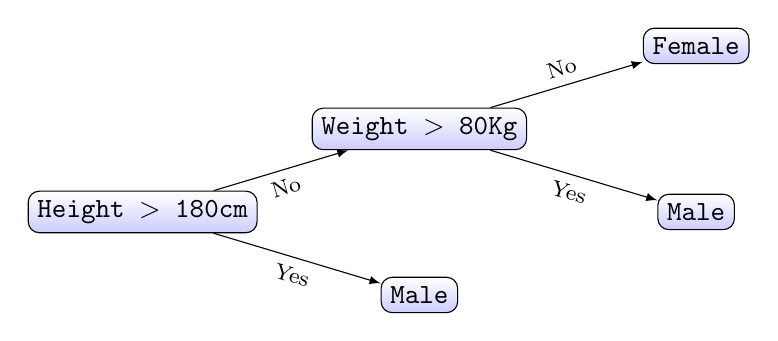
\begin{tikzpicture}
  [
    grow                    = right,
    sibling distance        = 6em,
    level distance          = 10em,
    edge from parent/.style = {draw, -latex},
    every node/.style       = {font=\footnotesize},
    sloped
  ]
  %\node [root] {Height $>$ 180}
  \node [env] {Height $>$ 180cm}
  		child { node [env] {Male}
      		edge from parent node [below] {Yes} }  
      	child { node [env] {Weight $>$ 80Kg}
      		  	child { node [env] {Male}
      				edge from parent node [below] {Yes} }   
      		  	child { node [env] {Female}
      				edge from parent node [above] {No} }        				
      		edge from parent node [below] {No} };
\end{tikzpicture}
\caption{Decision tree}
\label{fig:decisiontree}
\end{figure}
A learned binary tree is actually a partitioning of the input space. You can think of each input variable as a dimension on a p-dimensional space. The decision tree split this up into rectangles (when p=2 input variables) or some kind of hyper-rectangles with more inputs.
New data is filtered through the tree and lands in one of the rectangles and the output value for that rectangle is the prediction made by the model. This gives you some feeling for the type of decisions that a CART model is capable of making, e.g.\ boxy decision boundaries.


The selection of which input variable to use and the specific split or cut-point is chosen using a greedy algorithm to minimize a cost function. Tree construction ends using a predefined stopping criterion, such as a minimum number of training instances assigned to each leaf node of the tree.


\subsection{Greedy splitting}
Creating a binary decision tree is actually a process of dividing up the input space. A greedy approach is used to divide the space called recursive binary splitting. This is a numerical procedure where all the values are lined up and different split points are tried and tested using a cost function. The split with the best cost (lowest cost because we minimize cost) is selected. All input variables and all possible split points are evaluated and chosen in a greedy manner (e.g. the very best split point is chosen each time).

For regression predictive modelling problems the cost function that is minimized to choose split points is the sum squared error across all training samples that fall within the rectangle:
\begin{equation*}
\sum(y-\mbox{prediction})^2
\end{equation*}
where $y$ is the output for the training sample and prediction is the predicted output for the rectangle.

For classification the cost function provides an indication of how ``pure" the leaf nodes are (how mixed the training data assigned to each node is). There are three commonly used impurity measures used in binary decision trees: Entropy, Gini index, and Classification Error.
\begin{align*}
\mbox{Entropy} &= - \sum_j p_j \log p_j \\
\mbox{Gini} &= 1 - \sum_j {p_j}^2 \\
\mbox{Classification Error} &= 1 - \max {p_j}
\end{align*}
where $p_j$ is the probability of class $j$.
The entropy is $0$ if all samples of a node belong to the same class, and the entropy is maximal if we have a uniform class distribution. In other words, the entropy of a node (consist of single class) is zero because the probability is $1$ and $\log (1) = 0$. Entropy reaches maximum value (i.e.\ 1) when all classes in the node have equal probability. Similar to entropy, the Gini index is maximal (i.e.\ 0.5) if the classes are perfectly mixed, for example, in a binary class.

We start at the tree root and split the data on the feature that results in the largest information gain. The Information Gain (IG) can be defined as follows:
\begin{equation*}
{IG}(D_p) = I(D_p) - \frac{N_{l}}{N_p}I(D_{l}) - \frac{N_{r}}{N_p}I(D_{r})
\end{equation*}
where $I$ could be entropy, Gini index, or classification error, $D_p$, $D_l$, and $D_r$ are the dataset of the parent, left and right child node.

%\href{http://www.bogotobogo.com/python/scikit-learn/scikt_machine_learning_Decision_Tree_Learning_Informatioin_Gain_IG_Impurity_Entropy_Gini_Classification_Error.php}{Example}

\begin{figure}
\centering
\begin{subfigure}{.4\textwidth}
\centering
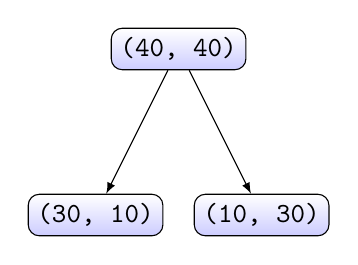
\begin{tikzpicture}
  [
    grow                    = down,
    sibling distance        = 6em,
    level distance          = 6em,
    edge from parent/.style = {draw, -latex},
    every node/.style       = {font=\footnotesize},
    sloped
  ]
  \node [env] {(40, 40)}
  		child { node [env] {(30, 10)}
      		edge from parent node [above] {} }  
      	child { node [env] {(10, 30)}      				
      		edge from parent node [below] {} };
%   \label{fig:informationgain1}
\end{tikzpicture}
\caption*{A}
\end{subfigure}
\qquad
\begin{subfigure}{.4\textwidth}
\centering
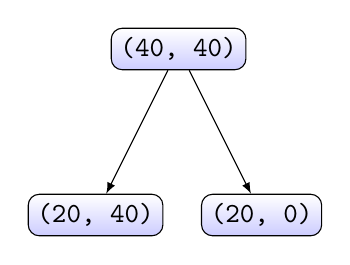
\begin{tikzpicture}
  [
    grow                    = down,
    sibling distance        = 6em,
    level distance          = 6em,
    edge from parent/.style = {draw, -latex},
    every node/.style       = {font=\footnotesize},
    sloped
  ]
  \node [env] {(40, 40)}
  		child { node [env] {(20, 40)}
      		edge from parent node [above] {} }  
      	child { node [env] {(20, 0)}      				
      		edge from parent node [below] {} };
%   \label{fig:informationgain2}
\end{tikzpicture}
\caption*{B}
\end{subfigure}
\caption{Information Gain - Example}
\label{fig:informationgain}
\end{figure}

As per the Information gain example in Figure~\ref{fig:informationgain} -
\begin{align*}
\mbox{Classification Error} &= 1 - \max p_j \\
A: I_E(D_p) &= 1 - \frac{40}{80} = 0.5\\
A: I_E(D_l)  &= 1 - \frac{30}{40} = 0.25\\
A: I_E(D_r)  &= 1 - \frac{30}{40} = 0.25\\
IG_{E} &= 0.5 - \frac{40}{80} * 0.25 - \frac{40}{80} * 0.25 = 0.25 \\
B: I_E(D_l)  &= 1 - \frac{40}{60} = \frac{1}{3}\\
B: I_E(D_r)  &= 1 - \frac{20}{20} = 0\\
IG_{E} &= 0.5 - \frac{60}{80} * \frac{1}{3} - \frac{20}{80} * 0 = 0.25 \\
\end{align*}
The information gains using the classification error as a splitting criterion are the same (0.25) in both cases A and B.
\begin{align*}
\mbox{Gini index} &= 1 - \sum_j {p_j}^2 \\
A: I_E(D_p) &= 1 - \bigg(\Big(\frac{40}{80}\Big)^2 + \Big(\frac{40}{80}\Big)^2\bigg) = 0.5\\
A: I_E(D_l)  &= 1 - \bigg(\Big(\frac{30}{40}\Big)^2 + \Big(\frac{10}{40}\Big)^2\bigg) = 0.375\\
A: I_E(D_r)  &= 1 - \bigg(\Big(\frac{10}{40}\Big)^2 + \Big(\frac{30}{40}\Big)^2\bigg) = 0.375\\
IG_{G} &= 0.5 - \frac{40}{80} * 0.25 - \frac{40}{80} * 0.25 = 0.25 \\
B: I_E(D_l)  &= 1 - \bigg(\Big(\frac{20}{60}\Big)^2 + \Big(\frac{40}{60}\Big)^2\bigg) = 0.44\\
B: I_E(D_r)  &= 1 - \bigg(\Big(\frac{20}{20}\Big)^2 + \Big(\frac{0}{20}\Big)^2\bigg) = 0\\
IG_{G} &= 0.5 - \frac{60}{80} * 0.44 - \frac{20}{80} * 0 = 0.17 \\
\end{align*}
The information gains using the Gini index favors the split B.
\begin{align*}
\mbox{Entropy} &= - \sum_j p_j \log p_j\\
A: I_E(D_p) &= - \bigg(\Big(\frac{40}{80}\Big) \log \Big(\frac{40}{80}\Big) + \Big(\frac{40}{80}\Big) \log \Big(\frac{40}{80}\Big)\bigg) = 1\\
A: I_E(D_l)  &= - \bigg(\Big(\frac{30}{40}\Big) \log \Big(\frac{30}{40}\Big) + \Big(\frac{10}{40}\Big) \log \Big(\frac{10}{40}\Big)\bigg) = 0.81\\
A: I_E(D_r)  &= - \bigg(\Big(\frac{10}{40}\Big) \log \Big(\frac{10}{40}\Big) + \Big(\frac{30}{40}\Big) \log \Big(\frac{30}{40}\Big)\bigg) = 0.81\\
IG_{H} &= 0.5 - \frac{40}{80} * 0.25 - \frac{40}{80} * 0.25 = 0.25 \\
B: I_E(D_l)  &= - \bigg(\Big(\frac{20}{60}\Big) \log \Big(\frac{20}{60}\Big) + \Big(\frac{40}{60}\Big) \log \Big(\frac{40}{60}\Big)\bigg) = 0.92\\
B: I_E(D_r)  &= - \bigg(\Big(\frac{20}{20}\Big) \log \Big(\frac{20}{20}\Big) + \Big(\frac{0}{20}\Big) \log \Big(\frac{0}{20}\Big)\bigg) = 0\\
IG_{H} &= 1 - \frac{60}{80} * 0.92 - \frac{20}{80} * 0 = 0.31 \\
\end{align*}
The information gains using the entropy criterion favors B.

%For classification the \emph{Gini} index function is used which provides an indication of how ``pure" the leaf nodes are (how mixed the training data assigned to each node is).
%\begin{equation*}
%G = \sum(p_k(1-p_k))
%\end{equation*}
%where $G$ is the Gini index over all classes, $p_k$ are the proportion of training instances with class $k$ in the rectangle of interest. A node that has all classes of the same type (perfect class purity) will have $G=0$, where as a $G$ that has a $50-50$ split of classes for a binary classification problem (worst purity) will have a $G=0.5$.

\subsection{Stopping criterion}
The recursive binary splitting procedure described above needs to know when to stop splitting as it works its way down the tree with the training data.
The most common stopping procedure is to use a minimum count on the number of training instances assigned to each leaf node. If the count is less than some minimum then the split is not accepted and the node is taken as a final leaf node.

The count of training members is tuned to the dataset, e.g.\ 5 or 10. It defines how specific to the training data the tree will be. Too specific (e.g.\ a count of 1) and the tree will overfit the training data and likely have poor performance on the test set.

\subsection{Pruning the tree}
The stopping criterion is important as it strongly influences the performance of your tree. You can use pruning after learning your tree to further lift performance.
The complexity of a decision tree is defined as the number of splits in the tree. Simpler trees are preferred. They are easy to understand (you can print them out and show them to subject matter experts), and they are less likely to overfit your data.

The fastest and simplest pruning method is to work through each leaf node in the tree and evaluate the effect of removing it using a hold-out test set. Leaf nodes are removed only if it results in a drop in the overall cost function on the entire test set. You stop removing nodes when no further improvements can be made.

More sophisticated pruning methods can be used such as cost complexity pruning (also called weakest link pruning) where a learning parameter (alpha) is used to weigh whether nodes can be removed based on the size of the sub-tree.

\section{Bootstrapping}
In machine learning, the \emph{bootstrap} method refers to random sampling with replacement. This sample is referred to as a resample. 
This allows the model or algorithm to get a better understanding of the various biases, variances and features that exist in the resample. Taking a sample of the data allows the resample to contain different characteristics than it might have contained as a whole.

The reason to use the bootstrap method is because it can test the stability of a solution. By using multiple sample data sets and then testing multiple models, it can increase robustness. Perhaps one sample data set has a larger mean than another, or a different standard deviation. This might break a model that was overfit, and not tested using data sets with different variations. Bootstrapping is used in both Bagging and Boosting.

\section{Bagging}
Bagging refers to bootstrap aggregation. Bagging predictors is a method for generating multiple versions of a predictor and using these to get an aggregated predictor.
What Bagging does is help reduce variance from models that are might be very accurate, but only on the data they were trained on. This is also known as overfitting. Overfitting is when a function fits the data too well. Typically this is because the actual equation is much too complicated to take into account each data point and outlier. For example, decision tree like CART has high variance.
Bagging gets around this by creating it's own variance amongst the data by sampling and replacing data while it tests multiple hypothesis (models). In turn, this reduces the noise by utilizing multiple samples that would most likely be made up of data with various attributes (median, average, etc).

Once each model has developed a hypothesis. The models use voting for classification or averaging for regression. This is where the `Aggregating' in `Bootstrap Aggregating' comes into play. Each hypothesis has the same weight as all the others. When we later discuss boosting, this is one of the places the two methodologies differ.
Essentially, all these models run at the same time, and vote on which hypothesis is the most accurate. This helps to decrease variance i.e.\ reduce the overfit.
Bagging is the application of the Bootstrap procedure to a high-variance machine learning algorithm, typically decision trees.

Let's assume we have a sample dataset of 1000 instances and we are using the CART algorithm. Bagging of the CART algorithm would work as follows:
\begin{enumerate} \addtolength{\itemsep}{-0.5\baselineskip}
\item Create many (e.g. 100) random sub-samples of our dataset with replacement.
\item Train a CART model on each sample.
\item Given a new dataset, calculate the average prediction from each model.
\end{enumerate}
For example, if we had 5 bagged decision trees that made the following class predictions for a in input sample: blue, blue, red, blue and red, we would take the most frequent class and predict blue.

When bagging with decision trees, we are less concerned about individual trees overfitting the training data. For this reason and for efficiency, the individual decision trees are grown deep (e.g. few training samples at each leaf-node of the tree) and the trees are not pruned. These trees will have both high variance and low bias. These are important characterize of sub-models when combining predictions using bagging.

The only parameters when bagging decision trees is the number of samples and hence the number of trees to include. This can be chosen by increasing the number of trees on run after run until the accuracy begins to stop showing improvement (e.g.\ on a cross validation test harness). Very large numbers of models may take a long time to prepare, but will not overfit the training data.
Just like the decision trees themselves, Bagging can be used for classification and regression problems.

\subsection{Random forest}
Random Forests are an improvement over bagged decision trees. A problem with decision trees like CART is that they are greedy. They choose which variable to split on using a greedy algorithm that minimizes error. As such, even with Bagging, the decision trees can have a lot of structural similarities and in turn have high correlation in their predictions.

Combining predictions from multiple models in ensembles works better if the predictions from the sub-models are uncorrelated or at best weakly correlated. Random forest changes the algorithm for the way that the sub-trees are learned so that the resulting predictions from all of the sub-trees have less correlation.

It is a simple tweak. In CART, when selecting a split point, the learning algorithm is allowed to look through all variables and all variable values in order to select the most optimal split-point. The random forest algorithm changes this procedure so that the learning algorithm is limited to a random sample of features of which to search.

The number of features that can be searched at each split point ($m$) must be specified as a parameter to the algorithm. You can try different values and tune it using cross validation.
\begin{enumerate} \addtolength{\itemsep}{-0.5\baselineskip}
\item For classification a good default is: $m = \sqrt{p}$
\item For regression a good default is: $m = p/3$
\end{enumerate}
where m is the number of randomly selected features that can be searched at a split point and p is the number of input variables. For example, if a dataset had 25 input variables for a classification problem, then:
\begin{enumerate} \addtolength{\itemsep}{-0.5\baselineskip}
\item $m = \sqrt{25}$
\item $m = 5$
\end{enumerate}

\subsubsection{Hyperparameters}
In the case of a random forest, hyperparameters include:
\begin{enumerate}
\item \texttt{n\_estimators} = number of trees in the foreset
\item \texttt{max\_features} = max number of features considered for splitting a node
\item \texttt{max\_depth} = max number of levels in each decision tree
\item \texttt{min\_samples\_split} = min number of data points placed in a node before the node is split
\item \texttt{min\_samples\_leaf} = min number of data points allowed in a leaf node
\item \texttt{bootstrap} = method for sampling data points (with or without replacement)
\end{enumerate}

\section{Boosting}
Boosting refers to a group of algorithms that utilize weighted averages to make weak learners into stronger learners. Unlike bagging that had each model run independently and then aggregate the outputs at the end without preference to any model. Boosting is all about `teamwork'. Each model that runs, dictates what features the next model will focus on.
Boosting also requires bootstrapping. However, there is another difference here. Unlike in bagging, boosting weights each sample of data. This means some samples will be run more often than others.

When boosting runs each model, it tracks which data samples are the most successful and which are not. The data sets with the most misclassified outputs are given heavier weights. These are considered to be data that have more complexity and requires more iterations to properly train the model.
During the actual classification stage, there is also a difference in how boosting treats the models. In boosting, the model's error rates are kept track of because better models are given better weights.
That way, when the `voting' occurs, unlike in bagging, the models with better outcomes have a stronger pull on the final output.

Boosting and bagging are both great techniques to decrease variance. Ensemble methods generally out perform a single model. There are different reasons you would use one over the other. Bagging is great for decreasing variance when a model is overfit. However, boosting is much more likely to be a better pick of the two methods. Boosting also is much more likely to cause performance issues. It is also great for decreasing bias in an underfit model. 


Boosting algorithms, such as AdaBoost, are iterative algorithms that place different weights on the training distribution each iteration. After each iteration boosting increases the weights associated with the incorrectly classified examples and decreases the weights associated with the correctly classified examples. This forces the learner to focus more on the incorrectly classified examples in the next iteration. Because rare classes/cases~\cite{DBLP:journals/sigkdd/Weiss04} are more error-prone than common classes/cases, it is reasonable to believe that boosting may improve their classification performance because, overall, it will increase the weights of the examples associated with these rare cases/classes. Note that because boosting effectively alters the distribution of the training data, one could consider it a type of advanced sampling technique.

\subsection{Additive model}
These models are fit by minimizing a loss function averaged over the training data, such as squared-error or a likelihood-based loss function,
\begin{align*}
\min_{\{\beta_m,\gamma_m\}} \sum_{i=1}^{N} L(y_i, f(x_i)) & \\
\mbox{where} \quad f(x) &= \sum_{m=1}^{M} \beta_m \, b(x;\gamma_m)
\end{align*}
where $\beta_m, m=1,2,\cdots,M$ are the expansion coefficients, and $b(x;\gamma) \in \mathbb{R}$ are usually simple functions of the multivariate argument $x$, characterized  by a set of parameters $\gamma$.  

The above function requires computationally intensive numerical optimization techniques. A simple alternative is to solve the subproblem of fitting just a single basis at a time. This is described in the algorithm called  \emph{forward stage-wise additive modelling}.
\begin{algorithm}[h]
\caption{Forward stage-wise additive modelling}
\begin{enumerate}
\item Initialize $f_0(x) = 0$.
\item For $m = 1$ to $M$:
	\begin{enumerate}
	\item Compute
		\begin{align*}
		(\beta_m,\gamma_m) &= \argmin_{\beta,\gamma} \sum_{i=1}^{N} L(y_i, f_{m-1}(x_i) + \beta \, b(x_i;\gamma))
		\end{align*}
	\item Set $f_m(x) = f_{m-1}(x) + \beta_m \, b(x;\gamma_m)$
	\end{enumerate}
\end{enumerate}
\end{algorithm}

\subsection{AdaBoost}
AdaBoost is equivalent to forward stage-wise additive modelling using the loss function:
\begin{align*}
L(y, f(x)) &= \exp{(-y f(x))} \\
\end{align*}

\subsection{XGBoost}

%% First enumerated chapter
%%-------------------------------------------------------------------------------
%\chapter{Learning To Rank}
%
%If you run an e-commerce website a classical problem is to rank your product offering in the search page in a way that maximises the probability of your items being sold. For example if you are selling shoes you would like the first pair of shoes in the search result page to be the one that is most likely to be bought.
%
%Thanks to the widespread adoption of machine learning it is now easier than ever to build and deploy models that automatically learn what your users like and rank your product catalog accordingly.
%
%Imagine you have an e-commerce website and that you are designing the algorithm to rank your products in your search page. What will be the first item that you display? The one with the best reviews? The one with the lowest price? Or a combination of both? The problem gets complicated pretty quickly.
%
%\section{PageRank}
%PageRank (PR) is an algorithm used by Google Search to rank websites in their search engine results. PageRank was named after Larry Page, one of the founders of Google. PageRank is a way of measuring the importance of website pages. According to Google:
%
%"PageRank works by counting the number and quality of links to a page to determine a rough estimate of how important the website is. The underlying assumption is that more important websites are likely to receive more links from other websites."
%
%It is not the only algorithm used by Google to order search engine results, but it is the first algorithm that was used by the company, and it is the best-known.
%
%Numerous academic papers concerning PageRank have been published since Page and Brin's original paper [ref]. In practice, the PageRank concept may be vulnerable to manipulation. Research has been conducted into identifying falsely influenced PageRank rankings. The goal is to find an effective means of ignoring links from documents with falsely influenced PageRank.
%
%Other link-based ranking algorithms for Web pages include the HITS algorithm invented by Jon Kleinberg [ref], the IBM CLEVER project [ref], the TrustRank algorithm [ref] and the hummingbird algorithm [ref].
%
%
%\section{Approaches to learning to rank}
%Please refer `Learning to Rank for Information Retrieval' by Tie-Yan Liu
%\begin{enumerate}
%\item The pointwise approach - The input space of the pointwise approach contains the feature vector of each single document. The output space contains the relevance degree of each single document. The hypothesis space contains functions that take the feature vector of a document as the input and predict the relevance degree of the document. The loss function examines the accurate prediction of the ground truth label for each single document. In different pointwise ranking algorithms, ranking is modelled as regression, classification, and ordinal regression. Therefore the corresponding regression loss, classification loss, and ordinal regression loss are used as the loss function.
%
%Note that the pointwise approach does not consider the interdependency among documents, and thus the position of a document in the final ranked list is invisible to its loss function. Furthermore, the approach does not make use of the fact that some documents are actually associated with the same query. Considering that most IR evaluation measures are query-level and position-based, intuitively speaking, the pointwise approach has its limitations.
%
%\item The pairwise approach - The input space of the pairwise approach contains a pair of documents, both represented as feature vectors.
%The output space contains the pairwise preference (which takes values from \{1, -1\}) between each pair of documents. The ground truth label in the output space is usually defined in the following way. The hypothesis space contains bi-variate functions h that take a pair of documents as the input and output the relative order between them, i.e., $h(x_u, x_v) = 2 \cdot I_{f(x_u)>f(x_v)} - 1$. The loss function measures the inconsistency between $h(x_u,x_v)$ and
%the ground truth label $y_{u,v}$.
%Note that the loss function used in the pairwise approach only considers the relative order between two documents. When one looks at only a pair of documents, however, the position of the documents in the final ranked list can hardly be derived. Furthermore, the approach ignores the fact that some pairs are generated from the documents associated with the same query. Considering that most IR evaluation measures are query-level and position-based, intuitively speaking, there is still a gap between this approach and ranking for IR.
%
%\item The listwise approach - 
%\end{enumerate}
%
%\section{Evaluation metrics}
%DCG and NDCG
%
%% enumerated chapter
%%-------------------------------------------------------------------------------
%\chapter{CTR - Click Through Rate}

\chapter{Support vector machine}
Hyperplane that partitions the two classes:
\begin{align*}
y &= \vec{w}^T\vec{x} + b
\end{align*}
Hyperplanes over the support vectors:
\begin{align*}
\vec{w}^T\vec{x} + b &= +1 \\
\vec{w}^T\vec{x} + b &= -1 
\end{align*}
The best partition line is the line parallel and equidistant from the support vectors, where the distance between the support vectors is the maximum and the partition line separates the two classes well.
Subtraction the above two lines: 
\begin{align*}
\vec{w}^T(\vec{x_1} - \vec{x_2}) &= +2 \\
\frac{\vec{w}^T}{||\vec{w}||}(\vec{x}_1 - \vec{x}_2) &= \frac{2}{||\vec{w}||} 
\end{align*}
Distance between the support vectors is given as: $\frac{\vec{w}^T}{||\vec{w}||}(\vec{x}_1 - \vec{x}_2)$. Increasing the distance between them is equivalent to minimizing the term $\frac{2}{||\vec{w}||}$, i.e.\ maximizing the margins.
The criteria that the partition line separates the two classes well is given as: $y(\vec{w}^T\vec{x}_j + b) \geq 1 \, \forall{j}$. As squaring preserves the order of the values (monotonic), maximizing $\frac{2}{||\vec{w}||}$ is equivalent to minimizing $\frac{||\vec{w}||^2}{2}$. 
The resultant optimization problem is of the form:
%\begin{align*}
%\mbox{minimize} & \quad \frac{||w||^2}{2} \\
%\mbox{where}	  & \quad y(w^Tx_i + b) \geq 1 \quad \forall{i}
%\end{align*}
%The above optimization problem is in the form of a quadratic optimization problem and there are standard algorithms to solve it.
\begin{align*}
\min_{\vec{w},b} & \quad \frac{1}{2} ||\vec{w}||^2 \\
\mathrm{where} & \quad (\vec{w} \cdot \vec{x}_j + b)y_j \geq 1, \quad \forall j
\end{align*}
The Lagrangian is:
\begin{align*}
L(\vec{w},\alpha) & =  \frac{1}{2} ||\vec{w}||^2  - \sum_j \alpha_j [(\vec{w} \cdot \vec{x}_j + b)y_j - 1]
\end{align*}
Our goal now is to solve:
\begin{align*}
\min_{\vec{w},b} \, \max_{\vec{\alpha}\geq0} &= \frac{1}{2}||\vec{w}||^2 - \sum_j \alpha_j [(\vec{w} \cdot \vec{x}_j + b)y_j - 1] \quad \mathrm{(Primal)}
\end{align*}
Swapping min and max, as the \emph{Slater's condition} from convex optimization guarantees that these two optimization problems are equivalent.
\begin{align*}
\max_{\vec{\alpha}\geq0} \, \min_{\vec{w},b} &= \frac{1}{2}||\vec{w}||^2 - \sum_j \alpha_j [(\vec{w} \cdot \vec{x}_j + b)y_j - 1] \quad \mathrm{(Dual)}
\end{align*}
Let us solve for optimal $\vec{w}, b$ as a function of $\vec{\alpha}$: 
\begin{align*}
\frac{\partial L}{\partial \vec{w}} = \vec{w} - \sum_j \alpha_j y_j \vec{x}_j \quad & \rightarrow \quad \vec{w} = \sum_j \alpha_j y_j \vec{x}_j \\
\frac{\partial L}{\partial b} = - \sum_j \alpha_j y_j \quad & \rightarrow \quad \sum_j \alpha_j y_j = 0
\end{align*}
Substituting these values back in (and simplifying), we obtain: 
\begin{align*}
\max_{\vec{\alpha}\geq0, \sum_j \alpha_j y_j = 0} & \sum_j \alpha_j - \frac{1}{2} \sum_{i,j} y_iy_j\alpha_i\alpha_j (\vec{x_i}\cdot \vec{x_j}) \quad \mathrm{(Dual)}
\end{align*}
Once $\alpha$ is estimated from the optimization function, we obtain $\vec{w}, b$.
$\vec{w} = \sum_j \alpha_j y_j \vec{x}_j$ and $b = y_k - \vec{w}\cdot \vec{x}_k$, for any $k$ where $\alpha_k > 0$.
The steps used to obtain $b$ are:
\begin{align*}
y_k (\vec{w}\cdot \vec{x}_k + b) &= 1 \\
y_ky_k (\vec{w}\cdot \vec{x}_k + b) &= y_k \\
\vec{w}\cdot \vec{x}_k + b &= y_k
\end{align*}
The classification rule is then $y \leftarrow \mathrm{sign} (\vec{w}\cdot\vec{x}+b)$. Using the dual solution $y \leftarrow \mathrm{sign} \big[\sum_i\alpha_iy_i(\vec{x_i}\cdot \vec{x})+b\big]$, where $\vec{x}$ is the support vector.

\subsection{Kernel trick}
\begin{align*}
\max_{\vec{\alpha}\geq0, \sum_j \alpha_j y_j = 0} & \sum_j \alpha_j - \frac{1}{2} \sum_{i,j} y_iy_j\alpha_i\alpha_j K(\vec{x_i}\cdot \vec{x_j}) \\
K(\vec{x_i}\cdot \vec{x_j}) &= \Phi (\vec{x_i}) \cdot \Phi (\vec{x_j})
\end{align*}

\chapter{Stochastic Gradient Descent}
\section{Convex function}
A function $f$ is convex if $\text{dom} f$ is a convex set and Jensen's inequality holds:
\[ f(\theta x + (1-\theta) y) \leq \theta f(x) + (1-\theta) f(y) \quad \forall \, \theta \in [0,1]\]
\textbf{First-order condition:}
for (continuously) differentiable $f$, Jensen's inequality can be replaced with:
\[ f(y) \geq f(x) + \nabla f(x)^T (y -x) \quad \forall \, x,y \in \text{dom}(f)\]
Proof: From the definition of the convex function we have -
\begin{align*}
f(\theta x + (1-\theta) y) & \leq \theta f(x) + (1-\theta) f(y) \quad \forall \, \theta \in [0,1] \\
f(x + \theta (y-x)) & \leq f(x) + \theta (f(y) - f(x)) \\
f(y) - f(x) & \geq \frac{f(x + \theta (y-x)) - f(x)}{\theta} \\
f(y) - f(x) & \geq \frac{f(x + \theta (y-x)) - f(x)}{x +\theta (y-x) - x} \times (y-x) \\
f(y) - f(x) & \geq \nabla f(x)^T (y-x)
\end{align*}
\textbf{Second-order condition:}
for twice differentiable $f$, Jensen's inequality can be replaced with:
\[ \nabla^2 f(x) \succeq 0 \quad \forall \, x \in \text{dom}(f)\]

\section{Gradient Descent}
When $f$ is convex 
\[ f(y) \geq f(x) + \nabla f(x)^T (y -x) \quad \forall \, x,y \in \text{dom}(f)\]
Therefore, $w$ close to $w^{(t)}$, we have $f(w) \approx f(w^{(t)}) + \langle (w - w^{(t)}), \nabla f(w^{(t)}) \rangle$.
Hence we can minimize the approximation of $f(w)$. However, the approximation might become loose for $w$, which is far away from $w(t)$. Therefore, we would like to minimize jointly the distance between $w$ and $w(t)$ and the approximation of $f$ around $w(t)$. If the parameter $\eta$ controls the tradeoff between the two terms, we obtain the update rule
\[ w^{(t+1)} = \argmin_w \, \frac{1}{2}\norm{w-w^{(t)}} + \eta \Big(f(w^{(t)}) + \langle w - w^{(t)}, \nabla f(w^{(t)}) \rangle\Big)\]
Solving the preceding by taking the derivative with respect to $w$ and comparing it to zero yields the update rule
\[ w^{(t+1)} = w^{t} - \eta \nabla f(w^{t}) \]

\chapter{Neural network}
\begin{itemize}
\item Epochs - One Epoch is when an ENTIRE dataset is passed forward and backward through the neural network only ONCE. Since, one epoch is too big to feed to the computer at once we divide it in several smaller batches.
\item Batch Size - Total number of training examples present in a single batch.
\item Iterations - Iterations is the number of batches needed to complete one epoch.
\end{itemize}
Let's say we have 2000 training examples that we are going to use. We can divide the dataset of 2000 examples into batches of 500 then it will take 4 iterations to complete 1 epoch.

\begin{itemize}
\item Stochastic Gradient Descent - Often abbreviated SGD, is a variation of the gradient descent algorithm that calculates the error and updates the model for each example in the training dataset.

The update of the model for each training example means that stochastic gradient descent is often called an online machine learning algorithm.
\item Batch gradient descent - It is a variation of the gradient descent algorithm that calculates the error for each example in the training dataset, but only updates the model after all training examples have been evaluated.

One cycle through the entire training dataset is called a training epoch. Therefore, it is often said that batch gradient descent performs model updates at the end of each training epoch.
\item Mini-batch gradient descent - It is a variation of the gradient descent algorithm that splits the training dataset into small batches that are used to calculate model error and update model coefficients.

Implementations may choose to sum the gradient over the mini-batch or take the average of the gradient which further reduces the variance of the gradient.

Mini-batch gradient descent seeks to find a balance between the robustness of stochastic gradient descent and the efficiency of batch gradient descent. It is the most common implementation of gradient descent used in the field of deep learning.
\end{itemize}

\chapter{Convolutional neural network}
Neural network equations:
\begin{align*}
z^{[l]} &= W^{[l]}a^{[l-1]} + b^{[l]} \\
a^{[l]} &= g(z^{[l]})
\end{align*}
Convolutional layer hyperparameter:
\begin{itemize}\addtolength{\itemsep}{-0.5\baselineskip}
\item $f^{[l]}$: filter size
\item $p^{[l]}$: padding
\item $s^{[l]}$: stride
\item $\eta_c^{[l-1]}$: number of channels
\item $\eta_c^{[l]}$: number of filters
\item each filter is: $f^{[l]} \times f^{[l]} \times \eta_c^{[l-1]}$
\item activation: $a^{[l]} \rightarrow \eta_h^{[l]} \times \eta_w^{[l]} \times \eta_c^{[l]}$
\item weights: $f^{[l]} \times f^{[l]} \times \eta_c^{[l-1]} \times \eta_c^{[l]}$
\item bias: $\eta_c^{[l]}$
\item input: $\eta_h^{[l-1]} \times \eta_w^{[l-1]} \times \eta_c^{[l-1]}$
\item output: $\eta_h^{[l]} \times \eta_w^{[l]} \times \eta_c^{[l]}$
\end{itemize}
where,
\begin{align*}
\eta_h^{[l]} &= \floor*{\frac{\eta_h^{[l-1]} + 2p^{[l]} - f^{[l]}}{s^{[l]}} + 1} \\
\eta_w^{[l]} &= \floor*{\frac{\eta_w^{[l-1]} + 2p^{[l]} - f^{[l]}}{s^{[l]}} + 1}
\end{align*}
Pooling layer hyperparameter:
\begin{itemize}\addtolength{\itemsep}{-0.5\baselineskip}
\item f: filter size
\item s: stride
\item each filter is: $f^{[l]} \times f^{[l]} \times 1$
\item input: $\eta_h^{[l-1]} \times \eta_w^{[l-1]} \times \eta_c^{[l-1]}$
\item output: $\eta_h^{[l]} \times \eta_w^{[l]} \times \eta_c^{[l]}$
\end{itemize}
where,
\begin{align*}
\eta_h^{[l]} &= \floor*{\frac{\eta_h^{[l-1]} + 2p^{[l]} - f^{[l]}}{s^{[l]}} + 1} \\
\eta_w^{[l]} &= \floor*{\frac{\eta_w^{[l-1]} + 2p^{[l]} - f^{[l]}}{s^{[l]}} + 1} \\
\eta_c^{[l]} &= \eta_c^{[l-1]}
\end{align*}
Residual network has the following \emph{short cut}: $a^{[l+2]} = g(z^{[l+2]} + a^{[l]})$

\section{Why convolutional layer?}
The two main advantages are parameter sharing and sparsity of connection.
Consider the following convolutional neural network: 
\begin{align*}
\mathrm{Input} & :  [\eta_h^{[l-1]} \times \eta_w^{[l-1]} \times \eta_c^{[l-1]}] \\
& = [32 \times 32 \times 3] \\
\mathrm{Filter} & : [f^{[l]} \times f^{[l]} \times \eta_c^{[l-1]}] \times \eta_c^{[l]} \\
& = [5 \times 5 \times 3] \times 6 \\
\mathrm{Bias} & : \eta_c^{[l]} \\
& = 6 \\
\mathrm{Output} & : [\eta_h^{[l]} \times \eta_w^{[l]} \times \eta_c^{[l]}] \\
& = [28 \times 28 \times 6]
\end{align*}
For the above network, the number of parameters of a convolutional neural network and a generic neural network are:
\begin{enumerate}\addtolength{\itemsep}{-0.5\baselineskip}
\item Parameters in a convolutional neural network
\begin{align*}
[f^{[l]} \times f^{[l]} \times \eta_c^{[l-1]}] \times \eta_c^{[l]} +  \eta_c^{[l]} &\\
[5 \times 5 \times 3] \times 6 + 6 & = 456
\end{align*}
\item Parameters in a neural network
\begin{align*}
[\eta_h^{[l-1]} \times \eta_w^{[l-1]} \times \eta_c^{[l-1]}]  \times [\eta_h^{[l]} \times \eta_w^{[l]} \times \eta_c^{[l]}]  & \\
[32 \times 32 \times 3] \times [28 \times 28 \times 6] & \approx 14\mathrm{M}
\end{align*}
\end{enumerate}
The parameters of of a convolutional neural network are far less than a generic neural network.

\section{Triplet loss}
Triplet loss is used in the Siamese Neural Net (NN) for one shot learning.
The Triplet loss tries to bring close the Anchor (current record) with the Positive (A record that is in theory similar with the Anchor) as far as possible from the Negative (A record that is different from the Anchor).

\begin{align*}
\mathrm{Step 1:} \quad & \vert \vert f(A) - f(P) \vert \vert^2 \leq \vert \vert f(A) - f(N) \vert \vert^2 \\
& \mathrm{adding \, margin} \, \alpha \\
\mathrm{Step 2:} \quad & \vert \vert f(A) - f(P) \vert \vert^2 + \alpha \leq \vert \vert f(A) - f(N) \vert \vert^2 \\
\mathrm{Triplet \, loss:} \quad & \mathcal{L}(A,P,N) = \max(\vert \vert f(A) - f(P) \vert \vert^2 - \vert \vert f(A) - f(N) \vert \vert^2 + \alpha, 0)
\end{align*}

\chapter{Sequence models}
\section{Recurrence neural network}
Recurrence neural network equations:
\begin{align*}
z^{<t>} &= W_{za}a^{<t-1>} + W_{zx}x^{<t>} + b_{z} \\
a^{<t>} &= g_a(z^{<t>}) \\
\hat{y}^{<t>} &= g_y(W_{ya}a^{<t>} +b_{y})
\end{align*}
Simplified recurrence neural network notation:
\begin{align*}
a^{<t>} &= g_a(W_{a}[a^{<t-1>},x^{<t>}] + b_{a}) \\
\hat{y}^{<t>} &= g_y(W_{y}a^{<t>} +b_{y})
\end{align*}

Types of recurrence neural network architecture
\begin{itemize}\addtolength{\itemsep}{-0.5\baselineskip}
\item one-to-one: Standard neural network
\item one-to-many: Music/sequence generation
\item many-to-one: Sentiment classification
\item many-to-many: Name entity recognition
\item many-to-many (encoder-decoder architecture): Machine translation
\end{itemize}

\subsection{Vanishing or exploding gradient problem}
Vanishing or exploding gradient is the problem where the derivative either decreases or grows exponentially as a function of the number of layers. The exploding gradient problem can be addressed by clipping the gradients. However, solving the vanishing gradient is challenging.

The vanishing gradient problem is a difficulty found in training artificial neural networks with gradient-based learning methods and backpropagation. In such methods, each of the neural network's weights receives an update proportional to the partial derivative of the error function with respect to the current weight in each iteration of training. The problem is that in some cases, the gradient will be vanishingly small, effectively preventing the weight from changing its value. In the worst case, this may completely stop the neural network from further training. As one example of the problem cause, traditional activation functions such as the hyperbolic tangent function have gradients in the range (0, 1), and backpropagation computes gradients by the chain rule. This has the effect of multiplying n of these small numbers to compute gradients of the "front" layers in an n-layer network, meaning that the gradient (error signal) decreases exponentially with n while the front layers train very slowly. 


\subsection{Gated recurrent unit}
Gated recurrence unit (GRU) helps in long range interaction.
\begin{align*}
\tilde{c}^{<t>} &= \tanh(W_{c}[c^{<t-1>},x^{<t>}] + b_{c}) \\
\gamma_u     &= \sigma	(W_{u}[c^{<t-1>},x^{<t>}] + b_{u})\\
c^{<t>} &= \gamma_u \ast  \tilde{c}^{<t>} + (1 - \gamma_u) \ast c^{<t-1>} \\
a^{<t>} &= c^{<t>} \\
\hat{y}^{<t>} &= g_y(W_{y}a^{<t>} +b_{y})
\end{align*}
where the subscript $u$ stands for the update gate.

\subsection{Long short-term memory}
Long short-term memory (LSTM) helps in long range interaction.
\begin{align*}
\tilde{c}^{<t>} &= \tanh(W_{c}[a^{<t-1>},x^{<t>}] + b_{c}) \\
\gamma_u     &= \sigma	(W_{u}[a^{<t-1>},x^{<t>}] + b_{u})\\
\gamma_f      &= \sigma	(W_{f}[a^{<t-1>},x^{<t>}] + b_{f})\\
\gamma_o     &= \sigma	(W_{u}[a^{<t-1>},x^{<t>}] + b_{o})\\
c^{<t>} &= \gamma_u \ast  \tilde{c}^{<t>} + \gamma_f \ast c^{<t-1>} \\
a^{<t>} &= \gamma_o \ast  \tanh(c^{<t>}) \\
\hat{y}^{<t>} &= g_y(W_{y}a^{<t>} +b_{y})
\end{align*}
where the subscripts $u$, $f$ and $o$ stands for the update, forget and output gates, respectively.

\subsection{Bidirectional RNN}
\begin{align*}
{\overrightarrow{a}}^{<t>} &= g_{\overrightarrow{a}}(W_{{\overrightarrow{a}}}[{\overrightarrow{a}}^{<t-1>},x^{<t>}] + b_{{\overrightarrow{a}}}) \\
{\overleftarrow{a}}^{<t>} &= g_{\overleftarrow{a}}(W_{{\overleftarrow{a}}}[{\overleftarrow{a}}^{<t-1>},x^{<t>}] + b_{{\overleftarrow{a}}}) \\
\hat{y}^{<t>} &= g_y(W_{y}[\overrightarrow{a}^{<t>}, \overleftarrow{a}^{<t>}] +b_{y})
\end{align*}

\chapter{Regression}
In linear regression we wish to fit a function (model) in this form:
\begin{align*}
\hat{Y} = \beta_0 + \beta_1 X_1  + \beta_2 X_2 + \cdots + \beta_n X_n
\end{align*}
where $X_i$ is the vector of features, and $\beta_i$ are the coefficients we wish to learn.

Having more features may seem like a perfect way for improving the accuracy of our trained model (reducing the loss) - because the model that will be trained will be more flexible and will take into account more parameters. On the other hand, we need to be extremely careful about overfitting the data. As we know, every dataset has noisy samples. 
The inaccuracies can lead to a low-quality model if not trained carefully. The model might end up memorizing the noise instead of learning the trend of the data.

Because overfit is an extremely common issue in many machine learning problems, there are different approaches to solving it. The main concept behind avoiding overfit is simplifying the models as much as possible. Simple models do not (usually) overfit. On the other hand, we need to pay attention the to gentle trade-off between overfitting and underfitting a model.

There is a gentle trade-off between fitting the model, but not overfitting it. 
One of the most common mechanisms for avoiding overfit is called regularization. Regularized machine learning model, is a model that its loss function contains another element that should be minimized as well.
\section{Ridge regression}
Ridge regression is an extension for linear regression. It's basically a regularized linear regression model. 
\begin{align*}
L = \sum (\hat{Y}_i - Y_i)^2 + \lambda \sum {\beta_i}^2 
\end{align*}
The second element though, a.k.a the regularization term, sums over squared $\beta$ values and multiplies it by another parameter $\lambda$. The reason for doing that is to ``punish'' the loss function for high values of the coefficients $\beta$. By punishing the $\beta$ values we add a constraint to minimize them as much as possible.
The $\lambda$ parameter is a scalar that is learned as well, using cross validation.

Ridge regression enforces the $\beta$ coefficients to be lower, but it does not enforce them to be zero. That is, it will not get rid of irrelevant features but rather minimize their impact on the trained model.

\section{Lasso}
Lasso is another extension built on regularized linear regression, but with L1 norm. The loss function of Lasso is in the form:
\begin{align*}
L = \sum (\hat{Y}_i - Y_i)^2 + \lambda \sum |{\beta_i}| 
\end{align*}
The only difference from Ridge regression is that the regularization term is in absolute value. But this difference has a huge impact on the trade-off between bias and variance. Lasso method overcomes the disadvantage of Ridge regression by not only punishing high values of the coefficients $\beta$ but actually setting them to zero if they are not relevant. Therefore, you might end up with fewer features included in the model than you started with, which is a huge advantage.

\chapter{Clustering}

\section{K-means clustering}
The K-means clustering algorithm uses iterative refinement to produce a final result. The algorithm inputs are the number of clusters K and the data set. The data set is a collection of features for each data point. The algorithms starts with initial estimates for the K centroids, which can either be randomly generated or randomly selected from the data set. The algorithm then iterates between two steps:

\begin{enumerate}
\item Data assigment step: Each centroid defines one of the clusters. In this step, each data point is assigned to its nearest centroid, based on the squared Euclidean distance. More formally, if $c_i$ is the collection of centroids in set $C$, then each data point x is assigned to a cluster based on
\[ \argmin_{c_i \in C} \, \mbox{dist}(c_i,x)^2\]
where $\mbox{dist}(.)$ is the standard (L2) Euclidean distance. Let the set of data point assignments for each $i^{\mbox{th}}$ cluster centroid be $S_i$.
\item Centroid update step: In this step, the centroids are recomputed. This is done by taking the mean of all data points assigned to that centroid's cluster.
\[ c_i = \frac{1}{|S_i|}\sum_{x_i \in S_i}x_i\]
\end{enumerate}

The algorithm iterates between steps one and two until a stopping criteria is met (i.e., no data points change clusters, the sum of the distances is minimized, or some maximum number of iterations is reached).
This algorithm is guaranteed to converge to a result. The result may be a local optimum (i.e. not necessarily the best possible outcome), meaning that assessing more than one run of the algorithm with randomized starting centroids may give a better outcome.

The algorithm described above finds the clusters and data set labels for a particular pre-chosen K. To find the number of clusters in the data, the user needs to run the K-means clustering algorithm for a range of K values and compare the results. In general, there is no method for determining exact value of K, but an accurate estimate can be obtained using the following techniques.

One of the metrics that is commonly used to compare results across different values of K is the mean distance between data points and their cluster centroid. Since increasing the number of clusters will always reduce the distance to data points, increasing K will always decrease this metric, to the extreme of reaching zero when K is the same as the number of data points. Thus, this metric cannot be used as the sole target. Instead, mean distance to the centroid as a function of K is plotted and the ``elbow point'', where the rate of decrease sharply shifts, can be used to roughly determine K.

\chapter{Recommendations}
A recommender system is a technology that is deployed in the environment where \emph{items} (products, movies, events, articles) are to be recommended to \emph{users} (customers, visitors, app users, readers) or the opposite. Typically, there are many items and many users present in the environment making the problem hard and expensive to solve. Imagine a shop. Good merchant knows personal preferences of customers. Her/His high quality recommendations make customers satisfied and increase profits. In case of online marketing and shopping, personal recommendations can be generated by an artificial merchant: the recommender system.

\section{Knowledge based recommender systems}
Both users and items have attributes. The more you know about your users and items, the better results can be expected. 

Such attributes are very useful and data mining methods can be used to extract knowledge in forms of rules and patterns that are subsequently used for recommendation. For example, the item above is represented by several attributes that can be used to measure similarity of items. Even the long text description can be processed by advanced NLP tools. Then, recommendations are generated based on item similarity. When users are also described by similar attributes (e.g.\ text extracted from CVs of job applicants), you can recommend items based on user-item attributes similarities. Note that in this case we do not use past user interactions at all. This approach is therefore very efficient for so called ``cold start'' users and items. Those are typically new users and new items.

\section{Content based recommender systems}
Such systems are recommending items similar to those a given user has liked in the past, regardless of the preferences of other users. Basically, there are two different types of feedback.

\emph{Explicit} feedback is intentionally provided by users in form of clicking the ``like''/``dislike'' buttons, rating an item by number of stars, etc. In many cases, it is hard to obtain explicit feedback data, simply because the users are not willing to provide it. Instead of clicking ``dislike'' for an item which the user does not consider interesting, he/she will rather leave the web page or switch to another TV channel.

\emph{Implicit} feedback data, such as ``user viewed an item'', ``user finished reading the article'' or ``user ordered a product'', however, are often much easier to collect and can also help us to compute good recommendations.

Content based recommenders work solely with the past interactions of a given user and do not take other users into consideration. The prevailing approach is to compute attribute similarity of recent items and recommend similar items.

\section{Collaborative filtering}
Last group of recommendation algorithms is based on past interactions of the whole user-base. These algorithms are far more accurate than the algorithms described in previous sections, when a ``neighborhood'' is well defined and the interactions data are clean.

To construct a recommendation for a user, k-nearest neighbor users (with most similar ranked items) are examined. Then, top N extra items (non-overlapping with items ranked by the user) are recommended.

K-nearest neighbor algorithm is not only solution to collaborative filtering problem. The rule-based algorithm above uses `Apriori algorithm' to generate set of rules from the interaction matrix. The rules with a sufficient support are subsequently used to generate candidate items for recommendations.

Important difference between K-NN and rule based algorithms is the speed of learning and recall. Machine learning models operate in two phases. In the learning phase, model is constructed and in the recall phase, model is applied to new data. Rule based algorithms are expensive to train but their recall is fast. K-NN algorithms are just the opposite, therefore they are also called lazy learners. In recommender systems, it is important to update model frequently (after each user interaction), to be able to generate new recommendations instantly. Whereas lazy learners are easy to update, rule based models have to be retrained, which is particularly challenging in large production environments. However, rules can be visualized and it is great tool to inspect quality of data and problems in your database. 

\subsection{Matrix factorization}

% Topics in natural language processing
%-------------------------------------------------------------------------------
\chapter{Natural language processing}

\section{Introduction}
Topics in the area of natural language understanding:
\begin{enumerate}
\item Sentiment Analysis - Deriving sentiments in sentences (positive, negative, neutral), and also in articles. The future is to include emotions (attributes) in that, like the attributes now on Facebook posts - Love, Like, Angry, Surprised, Sad, Hilarious. These attributes make a lot more sense for sentiments going forward.

\item Text Summarization - Summarizing a single or many articles according to a particular theme.

\item Textual Entailment - Inferring directional causal relationships between textual fragments. This can be challenging in a long article.

\item Information Extraction - Find structured information from unstructured data, like entities, relationships, co-reference resolution. This at a basic level is very useful for algorithmic trading. An extension of this is a global form of extracting logic structures

\item Topic Segmentation - Topic Extraction (with regions). Normally, there will be overlapping regions.

\item Question Answering - Answer the questions to both closed (specific) and open questions (subjective). Answers to subjective questions is the main challenge for the likes of realistic Virtual Assistants.

\item Parsing - Parsing natural language generally in the form a tree. This involves hierarchical segmentation of the language involving the grammar rules.

\item Prediction - Given a short text, predict what happens next. The prediction problem is beginning to be targeted in vision, but it has never ever gained paths for realistic products. For closed and deterministic prediction, this can be a useful task for prediction of future events based on past evidences and analysis. This can be then very useful for finance sectors.

\item Part of Speech Tagging (POS) - Tagging words whether they are nouns, verbs or adjectives.

\item Translation - Translate one language to another. This can be very challenging given the nature of the language, and the grammar. Normally, under probabilistic models, this assumes that the underlying grammar is mostly the same, and thus, models normally fail for Sanskrit.

\item Query Expansion - Expand query in possible ways for making the search results more meaningful. This is normally an issue with search engines, where people do not know what all keywords (or query sentences) to include to cover the entire gamut of relevancy.

\item Argumentation Mining - Evolving field of NLP, where one wants to analyse discussions and arguments.

\item Interestingness - Most interesting portion of text in an article. This can be done very much on the same lines as in images, where one ranks the likeness of images.
\end{enumerate}

\section{Language model}
A statistical language model is a probability distribution over sequences of words. Given such a sequence, say of length $m$, it assigns a probability $P(w_{1},\ldots ,w_{m})$ to the whole sequence. 
In an \emph{n-gram} model, the probability $P(w_{1},\ldots ,w_{m})$ of observing the sentence $w_{1},\ldots ,w_{m}$ is approximated as
\[ P(w_{1},\ldots ,w_{m})=\prod _{{i=1}}^{m}P(w_{i}\mid w_{1},\ldots ,w_{{i-1}})\approx \prod _{{i=1}}^{m}P(w_{i}\mid w_{{i-(n-1)}},\ldots ,w_{{i-1}}) \]
Here, it is assumed that the probability of observing the $i^{th}$ word $w_i$ in the context history of the preceding $i-1$ words can be approximated by the probability of observing it in the shortened context history of the preceding $n-1$ words ($n^{th}$ order Markov property). 
The conditional probability can be calculated from n-gram model frequency counts:
\[ P(w_{i}\mid w_{{i-(n-1)}},\ldots ,w_{{i-1}})={\frac {{\mathrm {count}}(w_{{i-(n-1)}},\ldots ,w_{{i-1}},w_{i})}{{\mathrm {count}}(w_{{i-(n-1)}},\ldots ,w_{{i-1}})}} \]
The words bigram and trigram language model denote \emph{n-gram} model language models with $n=2$ and $n=3$, respectively.

\chapter{Learning to rank}

At a high level, pointwise, pairwise and listwise approaches differ in how many documents you consider at a time in your loss function when training your model.
Pointwise approaches

Pointwise approaches look at a single document at a time in the loss function. They essentially take a single document and train a classifier / regressor on it to predict how relevant it is for the current query. The final ranking is achieved by simply sorting the result list by these document scores. For pointwise approaches, the score for each document is independent of the other documents that are in the result list for the query.

All the standard regression and classification algorithms can be directly used for pointwise learning to rank.
Pairwise approaches

Pairwise approaches look at a pair of documents at a time in the loss function. Given a pair of documents, they try and come up with the optimal ordering for that pair and compare it to the ground truth. The goal for the ranker is to minimize the number of inversions in ranking i.e. cases where the pair of results are in the wrong order relative to the ground truth.

Pairwise approaches work better in practice than pointwise approaches because predicting relative order is closer to the nature of ranking than predicting class label or relevance score. Some of the most popular Learning to Rank algorithms like RankNet, LambdaRank and LambdaMART [1] [2] are pairwise approaches.
Listwise approaches

Listwise approaches directly look at the entire list of documents and try to come up with the optimal ordering for it. There are 2 main sub-techniques for doing listwise Learning to Rank:
\begin{enumerate}
\item Direct optimization of IR measures such as NDCG. E.g. SoftRank [3], AdaRank [4]
\item Minimize a loss function that is defined based on understanding the unique properties of the kind of ranking you are trying to achieve. E.g. ListNet [5], ListMLE [6]
\end{enumerate}
Listwise approaches can get fairly complex compared to pointwise or pairwise approaches.

\chapter{Click-through rate}
Search engine advertising has become a significant element of the Web browsing experience. Choosing the right ads for the query and the order in which they are displayed greatly affects the probability that a user will see and click on each ad. This ranking has a strong impact on the revenue the search engine receives from the ads. Further, showing the user an ad that they prefer to click on improves user satisfaction. For these reasons, it is important to be able to accurately estimate the click-through rate of ads in the system. For ads that have been displayed repeatedly, this is empirically measurable, but for new ads, other means must be used.

Though there are many forms of online advertising, in this paper we will restrict ourselves to the most common model: pay-per-performance with a cost-per-click (CPC) billing, which means the search engine is paid every time the ad is clicked by a user (other models include cost-per-impression, where advertisers are charged according to the number of times their ad was shown, and cost-per-action, where advertisers are charged only when the ad dis- play leads to some desired action by the user, such as purchasing a product or signing up for a newsletter). Google, Yahoo, and Microsoft all primarily use this model.

In order to maximize ad quality (as measured by user clicks) and total revenue, most search engines today order their ads primarily based on expected revenue:
\[ E_{ad}[revenue] = p_{ad}(click) \times CPC_{ad} \]
Thus, to ideally order a set of ads, it is important to be able to accurately estimate the p(click) (CTR) for a given ad. For ads that have been shown to users many times (ads that have many impressions), this estimate is simply the binomial MLE (maximum likelihood estimation), \#clicks / \#impressions.

Whenever an ad is displayed on the search results page, it has some chance of being viewed by the user. The farther down the page an ad is displayed, the less likely it is to be viewed. As a simplification, we consider the probability that an ad is clicked on to be dependent on two factors: a) the probability that it is viewed, and b) the probability that it is clicked on, given that it is viewed:
\[ p(click|ad, pos) = p(click|ad, pos, seen)p(seen|ad, pos) \]
(Note that we are assuming that the probability that it is clicked on but not viewed is zero). We also make the simplifying assumptions that the probability an ad is clicked is independent of its position, given that it was viewed, and that the probability an ad is viewed is independent of the ad, given the position, and independent of the other ads shown:
\[ p(click|ad, pos) = p(click|ad, seen)p(seen| pos) \]
Let the CTR of an ad be defined as the probability it would be clicked if it was seen, or $p(click|ad, seen)$. From the CTR of an ad, and the discounting curve $p(seen|pos)$, we can then estimate the probability an ad would be clicked at any position. This is the value we want to estimate, since it provides a simple basis for comparison of competing ads.

For any ad that has been displayed a significant number of times, we can easily estimate its CTR. Whenever the ad was clicked, it was seen. Whenever the ad was not clicked, it may have been seen with some probability (e.g.\ heat map of search page viewership intensity for different ad position). Thus, the number of views of an ad is the number of times it was clicked, plus the number of times it was estimated to have been seen but not clicked. The CTR of the ad is simply the number of clicks divided by the total number of views.


Since our goal is to predict a real-value (the CTR of an $ad$), we cast it as a regression problem - that is, to predict the CTR given a set of features. We chose to use logistic regression~\cite{DBLP:conf/www/RichardsonDR07}, which is ideally suited for probabilities as it always predicts a value between 0 and 1:
\begin{align*}
CTR &= \frac{1}{1+e^{-Z}} \\
\mbox{where} \quad Z &= \sum_i w_i f_i(ad)
\end{align*}
where $f_i(ad)$ is the value of the $i^{th}$ feature for the ad, and $w_i$ is the learned weight for that feature. Features may be anything, such as the number of words in the title, the existence of a word, etc.

\chapter{Graphical models}
\href{https://medium.com/@neerajsharma_28983/intuitive-guide-to-probability-graphical-models-be81150da7a}{Graphical model}


\chapter{Miscellaneous} 

\begin{itemize}
\item Curse of dimensionality (\href{https://www.youtube.com/watch?v=5yzSv4jYMyI&list=PLgIPpm6tJZoShjm7r8Npia7CMsMlRWeuZ}{Youtube - ML Georgia Tech})
\item Regression - Lasso, quantile and cardinal
\item Recommendation
\item Detect anomalies - class imbalance - recognition problem 
\item Distributions, Hessian, Jacobian
\item R measure
\item Loss functions and Logistic regression
\item CNN - object detection
\item RNN - vanishing gradient
\item Boosting and XGBoost
\item Neural language model
\item Topic model - NMF and LDA. TopicRNN
\item Sequential model
\item Streaming data
\item Probabilistic Graphical Models (\href{https://medium.com/@neerajsharma_28983/intuitive-guide-to-probability-graphical-models-be81150da7a}{Blog})
\end{itemize}

%\hyperref[Data mining algorithms]{https://www.youtube.com/playlist?list=PLea0WJq13cnCS4LLMeUuZmTxqsqlhwUoe}

\chapter{Introduction to Bayesian methods and Conjugate priors}

\section{Think Bayesian and Statistics review}

\noindent
\textbf{Probability mass function:} 
A discrete random variable is a random variable whose range is finite or countably infinite. The probability mass function of a discrete random variable $X$ is 
\[ f_X(x) = P\{X=x\}\]
The mass function has two basic properties:
\begin{itemize}
\item $f_X(x) \geq 0$ for all $x$ in the state space
\item $\sum_x f_X(x) = 1$
\end{itemize}

\noindent
\textbf{Probability density function:} Let $X$ be  a  random  variable  whose  cumulative distribution function $F_X$ has a derivative. The  function $f_X$ satisfying
\[ F_X(x) = \int _{-\infty }^{x}f_{X}(t)\,dt \]
is called the probability density function and $X$ is called a continuous random variable.
By the fundamental theorem of calculus, ${F}'_X(x) = f_X(x)$. We can compute compute probabilities using
\[P\{a < X \leq b\} = F_X(b) - F_X(a) = \int _{a}^{b}f_{X}(t)\,dt\] 

\noindent
\textbf{Independence:} $X$ and $Y$ are independent if:
\begin{align*}
P(X,Y) &= P(X)P(Y) \\
\text{Joint} &= \text{Marginal} \times \text{Marginal}
\end{align*}

\noindent
\textbf{Conditional probability:} Probability of $X$ given that $Y$ happened:
\begin{align*}
P(X \vert Y) &= \frac{P(X,Y)}{P(Y)} \\
\text{Conditional} &= \frac{\text{Joint}}{\text{Marginal}}
\end{align*}

\noindent
\textbf{Chain rule:} 
\begin{align*}
P(X,Y) &= P(X \vert Y)P(Y) \\
P(X, Y, Z) &= P(X \vert Y, Z) P(Y \vert Z) P(Z) \\
P(X_1,X_2,\dots,X_N) &= \prod_{i=1}^{N}P(X_i \vert X_1,X_2,\dots,X_{i-1})
\end{align*}

\noindent
\textbf{Sum rule:} Marginalization
\begin{align*}
p(X) &= \int _{-\infty }^{\infty} p(X,Y) \, dY
\end{align*} 

\noindent
\textbf{Bayes theorem}
\begin{itemize}
\item $\theta$ - Parameters
\item $X$ - Observations
\end{itemize}
\begin{align*} 
P(\theta \vert X) &= \frac{P(\theta, X)}{P(X)} \\
&= \frac{P(X \vert \theta)P(\theta)}{P(X)} \\
\text{Posterior} &= \frac{\text{Likelihood} \times \text{Prior}}{\text{Evidence}} \\
& \propto \text{Likelihood} \times \text{Prior}
\end{align*}

\section{Bayesian approach to Statistics}
\noindent
\textbf{Frequentist approach:}
\begin{itemize}
\item $X$ is random and $\theta$ is fixed 
\item $\vert X \vert \gg \vert \theta \vert$
\item Maximum Likelihood: \[\hat{\theta} = \argmax_{\theta} P(X \vert \theta)\]
\end{itemize}

\noindent
\textbf{Bayesian approach:}
\begin{itemize}
\item $\theta$ is random and $X$ is fixed
\item For any $\vert X \vert$
\item Calculates the probability of parameters $\theta$ given the data $X$, using the Bayes theorem.
\[ P(\theta \vert X) =  \frac{P(X \vert \theta)P(\theta)}{P(X)} \]
\end{itemize}

\noindent
\textbf{Classification:}
\begin{itemize}
\item Training: 
\[P(\theta \vert X_{\text{tr}}, y_{\text{tr}}) =  \frac{P(y_{\text{tr}} \vert X_{\text{tr}},\theta)P(\theta)}{P(P(y_{\text{tr}} \vert X_{\text{tr}})}\]
\item Prediction:
\[P(y_{\text{ts}} \vert X_{\text{ts}}, X_{\text{tr}}, y_{\text{tr}}) = \int P(y_{\text{ts}} \vert X_{\text{ts}}, \theta) P(\theta \vert X_{\text{tr}}, y_{\text{tr}}) \, d\theta\]
\end{itemize}

\noindent
\textbf{Regularization:}
In Bayes theorem the prior $P(\theta)$ can be used as a regularizer.
\[ P(\theta \vert X) =  \frac{P(X \vert \theta)P(\theta)}{P(X)} \]

\noindent
\textbf{On-line learning:}
\begin{align*} 
P_k(\theta) = P(\theta \vert X_k) &= \frac{P(X_k \vert \theta)P_{k-1}(\theta)}{P(X_k)} \\
\text{New prior} = \text{Posterior} &= \frac{\text{Likelihood} \times \text{Prior}}{\text{Evidence}}
\end{align*}

\section{How to define a model}

\noindent
\textbf{Bayesian network:} We see that the event ``grass is wet'' has two possible causes: either the water sprinker is on or it is raining. Further the sprinkler is off when it is raining. 
\begin{figure}[h]
\centering
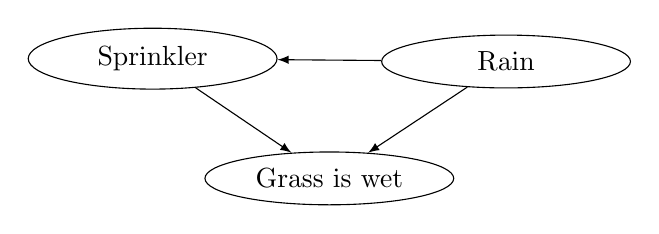
\begin{tikzpicture}[
  node distance=1cm and 0cm,
  mynode/.style={draw,ellipse,text width=2cm,align=center}
]
\node[mynode] (sp) {Sprinkler};
\node[mynode,below right=of sp] (gw) {Grass is wet};
\node[mynode,above right=of gw] (ra) {Rain};
\path (ra) edge[-latex] (sp)
(sp) edge[-latex] (gw) 
(gw) edge[latex-] (ra);
\end{tikzpicture}
\end{figure}
Note, we can't have interdependent variables in Bayesian network. For those cases we can either join random variables into one random variable or use Markov Random Fields (MRF).

\noindent
\textbf{Probabilistic model from BN:}
\begin{align*}
P(X_1,\dots,X_n) &= \prod_{k=1}^{n} P(X_k \vert \text{Pa}(X_k)) \\
\text{Pa}(G) &= \{R, S\} \\
P(S, R, G) &= P(G \vert S, R) P(S \vert R) P(R)
\end{align*}

\noindent
\textbf{Na\"{\i}ve Bayes:}
\begin{align*} 
P(c|f_1,f_2,\dots,f_N) &\propto  P(f_1,f_2,f_3,\dots,f_N,c) \\ 
&=  P(f_1|f_2,f_3,\cdots,f_N,c)P(f_2,f_3,\cdots,f_N,c) \\ 
&= P(f_1|f_2,f_3,\cdots,f_N,c)P(f_2|f_3,\cdots,f_N,c)P(f_3,\cdots,f_N,c) \\
&=  P(f_1|f_2,f_3,\cdots,f_N,c)P(f_2|f_3,\cdots,f_N,c) \cdots P(f_N|c)P(c) \\ 
&=  P(c)P(f_1|c)P(f_2|c) \cdots P(f_N|c) \\
&=  P(c)\prod_{i=1}^{N} P(f_i|c)
\end{align*}
\begin{align*} 
P(c|f_1,f_2,\cdots,f_N) &= P(c)\prod_{i=1}^{N} P(f_i|c)
\end{align*}

\begin{figure}[h]
\centering
  \tikz{
    % nodes
     \node[obs] (x) {$f$};%
     \node[latent,above=of x] (r) {$c$}; %
    % plate
     \plate [inner sep=.3cm,xshift=.02cm,yshift=.2cm] {plate1} {(x)} {N}; %
    % edges
     \edge {r} {x}  }
\caption{Plate notation}
\end{figure}

\section{Example: thief and alarm}
Imagine that you buy an alarm to a house to prevent thief from going into it. Either the thief goes into a house, and the alarm will go off and they will get, for example, SMS notification. However, the alarm may give a false alarm in case of an earthquake. Also, if there is a strong earthquake, the radio will report about it and so you get another source of them notification. Here's a graphical model for it. What is the general probability of the four and the variables, thief, alarm, earthquake, and the radio is given by the following formula. To fully define our model, we need to define these four probabilities.

\begin{figure}[h]
\centering
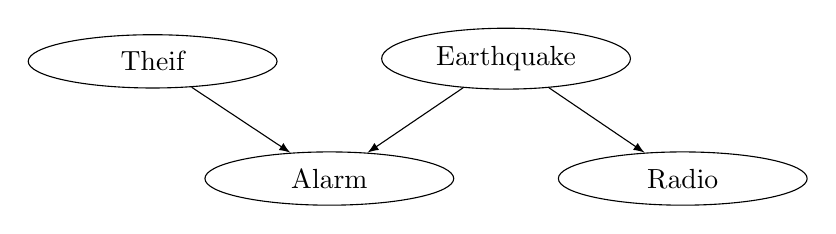
\begin{tikzpicture}[
  node distance=1cm and 0cm,
  mynode/.style={draw,ellipse,text width=2cm,align=center}
]
\node[mynode] (th) {Theif};
\node[mynode,below right=of th] (al) {Alarm};
\node[mynode,above right=of al] (eq) {Earthquake};
\node[mynode,below right=of eq] (ra) {Radio};
\path (th) edge[-latex] (al)
(eq) edge[-latex] (al) 
(eq) edge[-latex] (ra);
\end{tikzpicture}
\end{figure}

\begin{align*}
P(T,A,E,R) &= P(T)P(E)P(A \vert T,E) P(R \vert E)
\end{align*}


\begin{center}
\begin{tabular}{|| c | c ||}
 \hline
 Priors & \\ 
 \hline\hline
 $P(T)$ & $10^{-3}$ \\  
 $P(E)$ & $10^{-2}$ \\ 
 \hline
\end{tabular}
\end{center}

\begin{center}
\begin{tabular}{|| c | c c ||}
 \hline
 $P(A \vert T, E)$ & $\overline{E}$ &  $E$ \\ 
 \hline\hline
 $\overline{T}$ & $0$ & $1/10$ \\  
 $T$ & $1$ & $1$ \\ 
 \hline
\end{tabular}
\end{center}

\begin{center}
\begin{tabular}{|| c | c ||}
 \hline
 $P(R \vert E)$ & \\ 
 \hline\hline
 $\overline{E}$ & $0$ \\  
 $E$ & $1/2$ \\ 
 \hline
\end{tabular}
\end{center}

\begin{align*}
P(T \vert A) &= \frac{P(T, A)}{P(A)} \\
&= \frac{P(T, A, E) + P(T, A, \overline{E})}{P(T, A, E) + P(T, A, \overline{E}) + P(\overline{T}, A, E) + P(\overline{T}, A, \overline{E})} \\
&= \frac{P(T)P(E)P(A \vert T,E) + P(T)P(\overline{E})P(A \vert T,\overline{E})}
{P(T)P(E)P(A \vert T,E) + P(T)P(\overline{E})P(A \vert T,\overline{E}) + P(\overline{T})P(E)P(A \vert \overline{T},E) + P(\overline{T})P(\overline{E})P(A \vert \overline{T},\overline{E})}
\end{align*}

\begin{align*}
P(T \vert A, R) &= \frac{P(T, A, R)}{P(A, R)} \\
&= \frac{P(T, A, R, E) + P(T, A, R, \overline{E})}{P(T, A, R, E) + P(T, A, R, \overline{E}) + P(\overline{T}, A, R, E) + P(\overline{T}, A, R, \overline{E})}
\end{align*}

\section{Linear regression}
In linear regression, we want to feed a straight line into data. We feed it in the following way. You want to minimize the errors, and those are, the red line is the prediction and the blue points are the true values. And you want, somehow, to minimize those black lines. The line is usually found with so-called least squares problem. The prediction of each point is computed as $w$ transposed times $x_i$, where $x_i$ is our point. Then, we compute the total sum squares, that is, the difference between the prediction and the true value square. And we try to find the vector $w$ that minimizes this function. 

Let's see how this one works for the Bayesian perspective. Here's our model. We have three random variables, the weights, the data, and the target.
\begin{figure}[h]
\centering
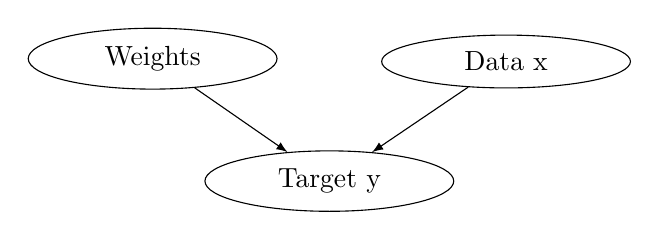
\begin{tikzpicture}[
  node distance=1cm and 0cm,
  mynode/.style={draw,ellipse,text width=2cm,align=center}
]
\node[mynode] (wg) {Weights};
\node[mynode,below right=of wg] (ty) {Target y};
\node[mynode,above right=of ty] (dx) {Data x};
\path (wg) edge[-latex] (ty)
(dx) edge[-latex] (ty);
\end{tikzpicture}
\end{figure}

We have three random variables, the weights, the data, and the target. We're not interested in modeling the data, so we can write down the joint probability of the weights and the target, given the data. This will be given by the following formula. 
\[P(w, y \mid X) = P(y \mid X, w)P(w)\]
It would be the probability of target given the weights of the data, and the probability of the weights. Now we need to define these two distributions. Let's assume them to be normal.
\begin{align*}
P(y \mid X, w) &= \mathcal{N}(y \mid w^{T}X, \sigma^{2} I) \\
P(w) &= \mathcal{N}(w \mid 0, \gamma^{2} I)
\end{align*}

Let's compute the posterior probability over the weights, given the data.
\begin{align*}
P(w \mid y, X) &= \frac{P(w, y \mid X)}{P(y \mid X)}
\end{align*}
We want to maximum of this posterior distribution with respect to the weights. Notice that the denominator does not depend on the weights, and so we can maximize only the numerator.
\begin{align*}
\argmax_w P(w \mid y, X) &= \argmax_w P(w, y \mid X) \\
&= \argmax_w P(y \mid X, w)P(w) \\
\argmax_w \log {P(w \mid y, X)} &= \argmax_w \, \big[  \log {P(y \mid X, w)} + \log {P(w)} \big] \\
&= \argmax_w \, \bigg[ \log C_1 \exp \Big( -\frac{1}{2} (y - w^TX)^T [\sigma^2 I]^{-1} (y - w^TX) \Big) + 
	 \log C_2 \exp \Big( -\frac{1}{2} w^T [\gamma^2 I]^{-1} w \Big) \bigg]\\
&= \argmax_w \, \Big[ \frac{1}{2\sigma^2} (y - w^TX)^T(y - w^TX) + \frac{1}{2\gamma^2} w^Tw \Big] \\
&= \argmax_w \, \norm{y - w^TX} + \lambda \norm{w}
\end{align*}
Notice the first term is sum of squares and the second term is a L2 regularizer.

\section{Likelihood}
Given a statistical probability mass function or density, say $f(x,\theta)$, where $\theta$ is an unknown parameter, the \emph{likelihood} is $f$ viewed as a function of $\theta$ for a fixed, observed value of $x$ of the random variable $X$. The probability density function is the continuous analogue of probability mass function.

Given the outcome $x$ of the random variable $X$, the likelihood function, which is a function of $\theta$, is given as:
\begin{equation*}
\mathcal{L}(\theta|x) = f_{\theta}(x) = P_{\theta}(X = x) = P(X = x \mid \theta) 
\end{equation*} 

For example -
\begin{enumerate} \addtolength{\itemsep}{-0.5\baselineskip}
\item Suppose we flip a coin with success probability of $\theta$
\item Recall that the mass function for $x$
\[ f(x, \theta) = {\theta}^x{(1-\theta)^{1-x}} \quad \mbox{for} \quad \theta \in [0, 1]\] 
where $x$ is either 0 (tails) or 1 (heads)
\item Suppose that the result is a head. The likelihood is 
\[ \mathcal{L}(\theta|1) = {\theta}^1{(1-\theta)^{1-1}} = \theta \quad \mbox{for} \quad \theta \in [0, 1]\]
\item Therefore, $\mathcal{L}(0.5|1)/\mathcal{L}(0.25|1) = 2$
\item There is twice as much evidence supporting the hypothesis that $\theta = 0.5$ to the hypothesis that $\theta = 0.25$
\end{enumerate}

\section{MLE and MAP estimation}
Maximum a posteriori (MAP) and maximum likelihood estimation (MLE) are stated as follows
\begin{align*}
\theta_{\mathcal{MAP}} &= \argmax_{\theta} P(\theta|X) \nonumber \\
									&= \argmax_{\theta} P(X|\theta) P(\theta)  \nonumber \\
\theta_{\mathcal{MLE}} &= \argmax_{\theta} P(X|\theta) \nonumber
\end{align*}
where $X$ is the input data and $\theta$ is the output parameter.

\section{Analytical inference}
There are many problems with Bayesian inference. In Bayes theorem, we have the likelihood times the prior over the evidence. However, what is the evidence? Imagine that they are working with images. For example, working with images of Van Gogh. You will have, for example, a Starry night, the Starry night over the Rhone. And if you model the probability of these images, you would also be able to draw new paintings that Van Gogh could have drawn. And so modelling this distribution is usually really hard. 

We'll try to come up with ideas how we can avoid computing the evidence. It is called a Maximum a posteriori principle. We try to find the value of the parameters that maximizes the posterior probability. In Bayes theorem note that evidence does not depend on theta. And so we can remove it. And so, by computing the Maximum a posteriori, we avoid conputing the evidence.


\section{Probability distributions}
\subsection{Normal distribution}
The probability density of the normal distribution is
\[\displaystyle \mathcal{N}(x\mid \mu ,\sigma ^{2})={\frac {1}{\sqrt {2\pi \sigma ^{2}}}}e^{-{\frac {(x-\mu )^{2}}{2\sigma ^{2}}}}\]
where $\mu$ is the mean or expectation of the distribution (and also its median and mode), $\sigma$ is the standard deviation, and $\sigma^{2}$ is the variance.

The multivariate normal distribution is said to be ``non-degenerate'' when the symmetric covariance matrix $\boldsymbol {\Sigma }$ is positive definite. In this case the distribution has density
\begin{align*}
\mathcal{N}(\mathbf {x} \mid \boldsymbol {\mu }, \boldsymbol {\Sigma })&={\frac{1}{\sqrt {(2\pi )^{k}|{\boldsymbol {\Sigma }}|}} \, {\exp \left(-{\frac {1}{2}}({\mathbf {x} }-{\boldsymbol {\mu }})^{\mathrm {T} }{\boldsymbol {\Sigma }}^{-1}({\mathbf {x} }-{\boldsymbol {\mu }})\right)}}
\end{align*}
where $\mathbf {x}$ is a real k-dimensional column vector and $|{\boldsymbol {\Sigma }}|\equiv \operatorname {det} {\boldsymbol {\Sigma }}$ is the determinant of ${\boldsymbol {\Sigma }}$. 
The equation above reduces to that of the univariate normal distribution if ${\boldsymbol {\Sigma }}$ is a $1\times 1$ matrix (i.e.\ a single real number). 

\subsection{Binomial Distribution}
\textbf{Problem:} A dice is rolled six times. What is the probability that we will get exactly two 3's? \newline
\textbf{Solution:} The probability of pattern $*,3,*,*,3,*$ is $\frac{5}{6}\times\frac{1}{6}\times\frac{5}{6}\times\frac{5}{6}\times\frac{1}{6}\times\frac{5}{6}$. We conclude that the probability of getting exactly two 3's is $\Mycomb[6]{2}\big(\frac{5}{6}\big)^4\big(\frac{1}{6}\big)^2$. \newline
\textbf{Definition:} We perform a trial independently for $n$ times, and on each trail an event we call `success' has probability $\theta$. Then the probability of $x$ successes out of $n$ trails is as follows:
\[f(x;n,\theta) = \Mycomb[n]{x}{\theta}^x(1-{\theta})^{n-x}\]

\begin{itemize}
\item $n$ trial
\item probability of success $\theta$
\item $x$ successes $\implies$ $n-x$ failures
\end{itemize}

\subsection{Multinomial Distribution}
\textbf{Problem:} Consider a die with 1 painted on three sides, 2 painted on two sides, and 3 painted on one side. If we roll this die ten times what is the probability we get five 1's, three 2's and two 3's? \newline
\textbf{Solution:} The probability of the pattern $1,1,1,1,1,2,2,2,3,3$ is $\big(\frac{3}{6}\big)^5 \times \big(\frac{2}{6}\big)^3 \times \big( \frac{1}{6}\big)^2$. We conclude that the probability of getting five 1's, three 2's and two 3's is $\Mycomb[10]{5}\Mycomb[5]{3}\big(\frac{3}{6}\big)^5\big(\frac{2}{6}\big)^3\big( \frac{1}{6}\big)^2$  i.e.\ $\frac{10!}{5!3!2!}\big(\frac{3}{6}\big)^5\big(\frac{2}{6}\big)^3\big( \frac{1}{6}\big)^2$. 
\newline
\textbf{Definition:} We see that if we have $k$ possible outcomes for our experiment with probabilities ${\theta}_1,\cdots,{\theta}_k$, then the probability of getting exactly $x_i$ outcomes of type $i$ in $n = {\sum}_{i=0}^{k}{x_i}$ trails is as follows: \newline \[f(x_1,\dots,x_k;n,{\theta}_1,\cdots,{\theta}_k) = \frac{n!}{x_1!x_2!\cdots x_k!}{\theta_1}^{x_1},\dots,{\theta_k}^{x_k}\]

\begin{itemize}
\item $n$ trial
\item $k$ bins
\item bin probabilities ${\theta}_1,\cdots,{\theta}_k$
\item $x_1$ items in $\text{bin-1}$, $x_2$ items in $\text{bin-2}$, $\dots \,$, $x_k$ items in $\text{bin-k}$
\end{itemize}

\subsection{Poisson Distribution}
We use Poisson distribution to approximate binomial distribution when $n$ is large.

\subsection{Bernoulli Distribution}
It is a special case of the Binomial distribution where a single trail is conducted $(n=1)$.
\[f(k;p) = p^k(1-p)^{1-k} \quad \text{for} \, k \in \{0,1\}\]
The distribution of heads $(k=1)$ and tails $(k=0)$ in coin tossing is an example of a Bernoulli distribution with $(p=1/2)$.

\subsection{Beta distribution}
Beta distribution is a type of statistical distribution, which has two free parameters. It is used as a prior distribution in Bayesian inference, due to the fact that it is the conjugate prior distribution for the binomial distribution, which means that the posterior distribution and the prior distribution are in the same family.

\subsection{Dirichlet distribution}
The Dirichlet distribution is a family of continuous multivariate probability distributions parameterised by a vector $\alpha$ of positive reals. It is the multivariate generalisation of the beta distribution. It is often used as the prior distribution in Bayesian inference and it is the conjugate prior of the categorical distribution and multinomial distribution.

\subsection{Gamma distribution}
Range $[0,\infty)$


\section{Conjugate prior}
In Bayesian probability theory, if the posterior distributions $p(\theta \mid x)$ are in the same probability distribution family as the prior probability distribution $p(\theta)$, the prior and posterior are then called conjugate distributions, and the prior is called a conjugate prior for the likelihood function $p(x \mid \theta)$.

Imagine you have a vectors of counts $\mathbf{n}$, that come from a multinomial distribution $\theta$. This multinomial comes from a Dirichlet distribution with a parameter $\alpha$.
Using chain rule we get $p(\mathbf{n}) = p(\mathbf{n}\mid \theta)p(\theta \mid \alpha)$. $p(\mathbf{n})$ is also Dirichlet distribution.

If $\theta \sim \text{Dir}(\alpha)$, $\mathbf{w} \sim \text{Dir}(\theta)$ and $n_k = \lvert{\{w_i: w_i =k \}}\rvert$, i.e. is count of $w_k$. 
\begin{align*}
p(\theta \mid \alpha, \mathbf{w}) &\propto p(\mathbf{w} \mid \theta) p(\theta \mid \alpha) \\
&\propto \prod_{k} {\theta}^{n_k} \prod_{k} {\theta}^{\alpha_k -1} \\
&\propto \prod_{k} {\theta}^{\alpha_k + n_k -1}
\end{align*}

\section{Expectation maximization}

\subsection{GMM}
\begin{align*}
p(x | \theta) &= \pi_1 \, \mathcal{N}(x\mid \mu_1 ,\Sigma_1) + \pi_2 \, \mathcal{N}(x\mid \mu_2 ,\Sigma_2) + \pi_3 \, \mathcal{N}(x\mid \mu_3 ,\Sigma_3) \\
\theta &= \{ \pi_1, \pi_2, \pi_3, \mu_1, \mu_2, \mu_3, \Sigma_1, \Sigma_2, \Sigma_3 \}
\end{align*}

Training GMM
\begin{align*}
\argmax_{\theta} \, p(X | \theta) &= \argmax_{\theta} \, \prod_{i=1}^{N}  p(x_i | \theta) \\
&= \argmax_{\theta} \, \prod_{i=1}^{N} ( \pi_1 \, \mathcal{N}(x_i\mid \mu_1 ,\Sigma_1) + \dots )
\end{align*}
subjected to $\, \sum_i \pi_i = 1; \, \pi_k \geq 0$ and $\Sigma_k \succ 0$.

\begin{figure}[h]
\centering
  \tikz{
    % nodes
     \node[obs] (x) {$x$};%
     \node[latent,left=of x] (r) {$t$}; %
     \edge {r} {x}  }
\caption{Latent variable}
\end{figure}

Introducing latent variable
\begin{align*}
p(t=c | \theta) &= \pi_c \\
p(x | t=c, \theta) &= \mathcal{N}(x\mid \mu_c ,\Sigma_c) \\
p(x | \theta) &= \sum_{c=1}^{N} p(x | t=c, \theta)p(t=c | \theta) 
\end{align*}

Parameter estimation
\begin{align*}
p(x | t=c, \theta) &= \mathcal{N}(x\mid \mu_c ,\sigma^{2}_{c}) \\
\mu_c  &= \frac{\sum_i p(t_i = c | x_i, \theta) x_i}{\sum_i p(t_i = c | x_i, \theta)} \\
\sigma^{2}_{c} &= \frac{\sum_i p(t_i = c | x_i, \theta) (x_i - \mu_c)^2}{\sum_i p(t_i = c | x_i, \theta)}
\end{align*}

\section{Variational inference vs.\ expectation maximization}
The difference lies mainly in that EM algorithm is a generic maximization algorithm that can be used for both frequentist inference and Bayesian inference. However, in contrast to the EM algorithm which only gives you a point estimate, it is always better for Bayesians if, hopefully, the whole posterior distribution is available. This is different from just obtaining one point estimate because then, you donot have any measure of uncertainty that your estimate conveys with it. This is where the variational Bayes (or variational inference, variational approximations) kicks in.

The difference of EM and VB is the kind of results they provide, EM is just a point, VB is a distribution. However, they also have similarities. EM and VB can both be interpreted as minimizing some sort of distance between the true value and our estimate, which is the Kullback-Leibler divergence.

So EM and VB are not really distinguished as to how complex they are used for is, but rather what kind of result it returns in the end.

\chapter{Maths}

\section{Hessian}

\section{Jacobian}

% Last pages for ToC
%-------------------------------------------------------------------------------
\newpage
% Include dots between chapter name and page number
\renewcommand{\cftchapdotsep}{\cftdotsep}
%Finally, include the ToC
\tableofcontents


\newpage
\bibliographystyle{abbrv}
\bibliography{ML} 
\end{document}

